\documentclass[a4paper, 11pt]{article}

\usepackage[top=112pt, bottom=112pt, left=90pt, right=85pt]{geometry}
\usepackage{geometry, amssymb, csquotes, amsmath, graphicx, mathtools, amsthm, calc, accents} 
\usepackage[hidelinks]{hyperref}
\usepackage[utf8]{inputenc}
\usepackage{xcolor}
\usepackage{todonotes}
% \usepackage[toc]{appendix}
%\usepackage{parskip}

\newcommand{\rem}[2][noinline]{\todo[#1, color=gray!20!white,size=\footnotesize]{\texttt{Rem}: #2}}
\newcommand{\doubletilde}[1]{\tilde{\raisebox{0pt}[0.85\height]{$\tilde{#1}$}}}
\newcommand{\tripletilde}[1]{\tilde{\raisebox{0pt}[0.85\height]{$\doubletilde{#1}$}}}

\newtheorem{prop}{Proposition}
\newtheorem{definition}{Definition}
\newtheorem{lemma}{Lemma}
\newtheorem{theor}{Theorem}
\newtheorem{cor}{Corollary}
\newtheorem{conjecture}{Conjecture}

\DeclareMathOperator\artanh{artanh}
\DeclareMathOperator\tr{tr}

\hypersetup{
  urlcolor = black,
  citecolor = black,
  pdftitle = {notes},
  pdfsubject = {notes},
  pdfpagemode = UseNone
}

% \hypersetup{
%     colorlinks=true,
%     linkcolor=blue,
%     filecolor=magenta,      
%     urlcolor=blue,
% }

\newcommand\underl[2]{\mathrel{\mathop{#2}\limits_{#1}}}

\title{\textbf{Exact computation of all variables' moments for linear gene expression models in tree-based compartmentalised neurons}}
\date{\today}
\begin{document}
\maketitle

\begin{abstract}
  Here we discuss the exact ways of finding the moments of the probability distribution directly from the {\it master equation} (ME). The main method is to find the asymptotic expansion (at least to the second order) of the {\it generating function}, which is directly related to the moments of the probability distribution. First we demonstrate the method on simple examples, then we derive the expressions (4,5,6) from \cite{PAULSSON2005157}, and then attempt to apply the method to simple neuron models. Note that the method gives the exact expressions for the moments, which is demonstrated for the simple examples by finding the generating function exactly.
\end{abstract}

\tableofcontents

\section{Introduction}
Often the probability distribution arises as a solution to the maser equation, and here we show how to find the moments of the unknown distribution without actually finding the distribution itself.
\subsection{The problem}

The master equation (ME) from \cite{PAULSSON2005157} reads as
\begin{equation} \label{full_Paulsson_ME}
  \begin{split} 
    \frac{dP_{n_1,n_2,n_3}(t)}{dt} = &\lambda_1^+\left[(N_1-n_1+1)P_{n_1-1,n_2,n_3}(t) - (N_1-n_1)P_{n_1,n_2,n_3}(t)\right]\\
    + & \lambda_1^-\left[(n_1+1)P_{n_1+1,n_2,n_3}(t) - n_1P_{n_1,n_2,n_3}(t)\right] \\
    + & \lambda_2\left[n_1P_{n_1,n_2-1,n_3}(t) - n_1P_{n_1,n_2,n_3}(t)\right]\\
    + & \tau_2^{-1}\left[(n_2+1)P_{n_1,n_2+1,n_3}(t) - n_2P_{n_1,n_2,n_3}(t)\right]\\
    + & \lambda_3\left[n_2P_{n_1,n_2,n_3-1}(t) - n_2P_{n_1,n_2,n_3}(t)\right]\\
    + & \tau_3^{-1}\left[(n_3+1)P_{n_1,n_2,n_3+1}(t) - n_3P_{n_1,n_2,n_3}(t)\right]
  \end{split}
\end{equation}
and takes into account activation/deactivation of $N_1$ independent copies of the same gene ($n_1$ is the number of active replicas of the gene at any given time), mRNA production and decay ($n_2$ is the number of mRNA molecules), and the production and decay of proteins ($n_3$ is the number of proteins).

In this introductory section we will show how to find the means, variances and correlations of all variables ${n_1, n_2, n_3}$ from the  probability distribution satisfying the equation (\ref{full_Paulsson_ME}) at stationarity\footnote{Note that the method is not limited to stationarity.}. Before that, we will demonstrate the method on two simple examples which are, in fact, identical, but we solve them differently to demonstrate the issues that arise from not embedding all the information to the master equation (which reduces dimensionality).

\subsection{Independent gene switching} \label{sec::independent_gene_switching}
\rem[inline]{I dont see very well what is the jump process in this case. A very natural way to describe a jump process is to give its infinitesimal generator $\mathbf A$ which is somehow the adjoint of the Fokker Planck equation. Formally, $\mathbf Af(x) = \lim\limits_{\delta\to 0}(E_x(f(X_\delta))-x)/\delta$
	
In your case, I'd say that \[(\mathbf Ah)(n) = \lambda_1^+1_{n<N_1}\left(f(n+1)-f(n)\right) + \lambda_1^-1_{n>0}\left(f(n-1)-f(n)\right) \]}
We will now demonstrate the approach by solving the problem of independent switching of $N_1$ gene replicas, for which the master equation is given by\footnote{Compare with the first two lines of (\ref{full_Paulsson_ME}).}
\begin{equation} \label{gene_switching_ME}
  \begin{split} 
    \frac{dP_{n_1}(t)}{dt} = &\lambda_1^+\left[(N_1-n_1+1)P_{n_1-1}(t) - (N_1-n_1)P_{n_1}(t)\right]\\
    + & \lambda_1^-\left[(n_1+1)P_{n_1+1}(t) - n_1P_{n_1}(t)\right],
  \end{split}
\end{equation}
where $n_1$ is the number of active genes.

The generating function of the distribution $P_{n_1}(t)$ is defined as
\begin{equation} \label{gen_func_def} 
  G(z_1; t) = \sum_{n_1=-\infty}^{\infty}P_{n_1}(t)z_1^{n_1}.
\end{equation}
Note that the moments of the probability distribution $P_{n_1}$ can be found from the derivatives of the generating function with respect to the corresponding variables, i.e.
\begin{align}
  \frac{\partial G(z_1; t)}{\partial z_1}\bigg\rvert_{z_1=1} &= \sum_{n_1=-\infty}^{\infty} n_1P_{n_1}(t) = \langle n_1\rangle(t); \label{1st_der_of_GF}\\
  \frac{\partial^2 G(z_1; t)}{\partial z_1^2}\bigg\rvert_{z_1=1} &= \sum_{n_1=-\infty}^{\infty} n_1(n_1-1)P_{n_1}(t) = \langle n_1\rangle^2(t) - \langle n_1\rangle(t)\label{2nd_der_of_GF}.
\end{align}

The generating function allows recasting the master equation (\ref{gene_switching_ME}) in a PDE form as follows. First, we multiply both sides of the ME (\ref{gene_switching_ME}) by $z_1^{n_1}$ and sum over $n_1$, which gives
\begin{equation*}
  \begin{split}
    \sum_{n_1=-\infty}^{\infty}\frac{dP_{n_1}(t)}{dt}z_1^{n_1} = &\lambda_1^+\sum_{n_1=-\infty}^{\infty}\left[(N_1-n_1+1)P_{n_1-1}(t) - (N_1-n_1)P_{n_1}(t)\right]z_1^{n_1}\\
    + & \lambda_1^-\sum_{n_1=-\infty}^{\infty}\left[(n_1+1)P_{n_1+1}(t) - n_1P_{n_1}(t)\right]z_1^{n_1}.
  \end{split}
\end{equation*}
Then, using the definition of the generating function (\ref{gen_func_def}) and the following identities
\begin{align*}
  & \sum_{n_1=-\infty}^{\infty}P_{n_1-1}(t)z_1^{n_1} = z_1\sum_{n_1=-\infty}^{\infty}P_{n_1-1}(t)z_1^{n_1-1} = z_1G(z_1;t);\\
  & \sum_{n_1=-\infty}^{\infty}P_{n_1+1}(t)z_1^{n_1} = \frac{1}{z_1}\sum_{n_1=-\infty}^{\infty}P_{n_1+1}(t)z_1^{n_1+1} = \frac{1}{z_1}G(z_1;t);\\
  & \sum_{n_1=-\infty}^{\infty}n_1P_{n_1}(t)z_1^{n_1} = z_1\frac{\partial}{\partial z_1}\sum_{n_1=-\infty}^{\infty}P_{n_1}(t)z_1^{n_1} = z_1\frac{\partial G(z_1; t)}{\partial z_1};\\
  & \sum_{n_1=-\infty}^{\infty}n_1P_{n_1-1}(t)z_1^{n_1} = z_1\frac{\partial}{\partial z_1}\sum_{n_1=-\infty}^{\infty}P_{n_1-1}(t)z_1^{n_1} = z_1\frac{\partial}{\partial z_1} \left(z_1G(z_1; t)\right);\\
  & \sum_{n_1=-\infty}^{\infty}n_1P_{n_1+1}(t)z_1^{n_1} = z_1\frac{\partial}{\partial z_1}\sum_{n_1=-\infty}^{\infty}P_{n_1+1}(t)z_1^{n_1} = z_1\frac{\partial}{\partial z_1} \left(\frac{1}{z_1}G(z_1; t)\right),
\end{align*}
we recast the equation (\ref{gene_switching_ME}) in the form of the following first-order partial differential equation (PDE)
\begin{equation*} \label{gene_switching_PDE}
  \frac{\partial G(z_1;t)}{\partial t} + (\lambda_1^+z_1 + \lambda_1^-)(z_1-1)\frac{\partial G(z_1;t)}{\partial z_1} = \lambda_1^+N_1(z_1-1)G(z_1;t),
\end{equation*}
which can be solved using the method of characteristics.

\subsubsection{Finding the generating function exactly}
For convenience we introduce new variable as
\begin{equation*}
  x_1 := z_1 - 1
\end{equation*}
and denote
\begin{equation*}
  \mathcal G(x_1; t) = G(z_1(x_1); t).
\end{equation*}
in terms of which the PDE (\ref{gene_switching_PDE}) becomes
\begin{equation} \label{gene_switching_PDE_x}
  \frac{\partial \mathcal G(x_1;t)}{\partial t} + (\lambda_1^+x_1 + \frac{1}{\tau_1})x_1\frac{\partial \mathcal G(x_1;t)}{\partial x_1} = \lambda_1^+N_1x_1\mathcal G(x_1;t),
\end{equation}
where $\tau_1 := (\lambda_1^+ + \lambda_1^-)^{-1}$.
The characteristic equations for the nonhomogeneous quasilinear PDE (\ref{gene_switching_PDE}) are given by
\begin{equation*}
  \begin{dcases}
    \dot t = \tau;\\
    \dot x_1 = \lambda_1^+x_1^2 + \frac{1}{\tau_1}x_1;\\
    \dot{\mathcal G} = \lambda_1^+N_1x_1\mathcal G,
  \end{dcases}
\end{equation*}
which have the following {\it first integrals}
\begin{align*}
  C_1& = -\left(P_\text{on}+\frac{1}{x_1}\right)\mathrm e^{t/\tau_1}\\
  C_2& = \left(\frac{-\mathrm e^{t/\tau_1}}{x_1P_{on}}\right)^{N_1}\mathcal G,
\end{align*}
where
\begin{equation*}
  P_\text{on} = \frac{\lambda_1^+}{\lambda_1^+ + \lambda_1^-} = \lambda_1^+\tau_1.
\end{equation*}

The general solution is given by\footnote{As an exercise one can check this solution by direct substitution to (\ref{gene_switching_PDE_x}).}
\begin{equation}\label{n1_general_solution}
  \mathcal G(x_1;t) = \left(-x_1P_{\text{on}}\mathrm e^{-t/\tau_1}\right)^{N_1}f\left(\left(P_{on}+\frac{1}{x_1}\right)\mathrm e^{t/\tau_1}\right),
\end{equation}
where $f(.)$ is an arbitrary function defined by the initial conditions.

Assuming that the initial number of active genes was $m$, i.e.
\begin{equation}\label{initial_condition}
  P_{n_1}(t=0) = \delta_{n_1,m} \implies \mathcal G(x_1; t=0) = (x_1+1)^m,
\end{equation}
we arrive to
\begin{equation*}
  f(\xi) = \left(\frac{\xi - P_\text{on}}{-P_{\text{on}}}\right)^{N_1}\cdot\left(\frac{1+\xi-P_\text{on}}{\xi-P_{\text{on}}}\right)^m,
\end{equation*}
from which (\ref{n1_general_solution}) reads as\footnote{Which, of course, can also be checked by the direct substitution to the PDE (\ref{gene_switching_PDE_x}) and the initial condition (\ref{initial_condition}).}
\begin{equation}\label{n1_special_solution}
  \mathcal G(x_1; t) = \left(x_1P_\text{on}\left(1-\mathrm e^{-t/\tau_1}\right)+1\right)^{N_1}\cdot\left(\frac{x_1\mathrm e^{-t/\tau_1}}{x_1P_\text{on}\left(1-\mathrm e^{-t/\tau_1}\right)+1} + 1\right)^m.
\end{equation}

%% \begin{equation}
%%   \mathcal G(x_1; t) = \left(x_1P_{\text{on}}\left(1-\mathrm e^{-t/\tau_1}\right)\right),
%% \end{equation}
%% and finally

Note that, as any generating function, $\mathcal G(x_1=0; t)=1$, and from (\ref{n1_special_solution}) it is clear that
\begin{equation}\label{binomial_gen_function}
  \lim_{t\to\infty}\mathcal G(x_1; t) = \left(1 + x_1P_\text{on}\right)^{N_1},
\end{equation}
which is expected, since (\ref{binomial_gen_function}) is the generating function of the binomial distribution with the probability of success $P_\text{on}$.

\subsubsection{Asymptotic expansion of the stationary solution} \label{switching_asymptotic_expansion}
Unfortunately, it is rarely possible to find the generating function exactly, but since the moments of the probability distribution only depend on the behaviour of $\mathcal G(x_1;t)$ in the vicinity of $x_1=0$, they can be obtained by means of an asymptotic expansion of $\mathcal G(x_1;t)$ around this point. In this section we exemplify this method on the model above, whose exact solution can be used for verification. To do this we substitute the function $\mathcal G$ in the form of its asymptotic expansion at $x_1=0$
\begin{equation}\label{two_compartment_hopping_expansion}
  \mathcal G(x_1;t) = 1 + \mathcal G^{(1)}(t)x_1 + \frac{1}{2}\mathcal G^{(2)}(t) x_1^2 + ... = 1 + \langle n_1\rangle(t) x_1 + \left[\langle n_1^2 \rangle(t)-\langle n_1\rangle(t)\right]x_1^2 + ...
\end{equation}
to the equation (\ref{gene_switching_PDE_x}), which at stationarity reads as
\begin{equation*}
  (\lambda_1^+x_1 + \frac{1}{\tau_1})x_1\frac{d\mathcal G(x_1)}{dx_1} = \lambda_1^+N_1x_1\mathcal G(x_1),
\end{equation*}
or equivalently
\begin{equation*}
  (P_{\text{on}}x_1 + 1)x_1\frac{d\mathcal G(x_1)}{dx_1} = P_{\text{on}}N_1x_1\mathcal G(x_1).
\end{equation*}
This substitution leads to
\begin{equation*}
  \left(P_{\text{on}}-\frac{1}{2}P_{\text{on}}N_1\right)\mathcal G^{(2)}x_1^3 + \left(\mathcal G^{(2)} + \mathcal G^{(1)}P_{\text{on}} - P_{\text{on}}N_1G^{(1)}\right)x_1^2 + \left(G^{(1)}-P_{\text{on}}N_1\right)x_1 = 0,
\end{equation*}
where the $\mathcal O(x^3)$ terms must be ignored, since we only do the expansion up to the second order. The unknown coefficients $\{\mathcal G^{(i)}\}$ are found by voiding all consecutive orders in $x$ up to two, which gives a non-degenerate system of two linear equations for two unknowns
\begin{equation*}
  \begin{dcases}
    G^{(1)}-P_{\text{on}}N_1 = 0\\
    \mathcal G^{(2)} - \mathcal G^{(1)}P_{\text{on}}(N_1-1) = 0,
  \end{dcases}
\end{equation*}
from which
\begin{equation*}
  \mathcal G^{(1)} = P_{\text{on}}N_1; \qquad     \mathcal G^{(2)} = P_{\text{on}}^2N_1(N_1-1).
\end{equation*}
Noticing that, as clear from (\ref{1st_der_of_GF}), (\ref{2nd_der_of_GF}) and the expansion (\ref{two_compartment_hopping_expansion}),
\begin{equation*}
  \mathcal G^{(1)} = \langle n_1 \rangle; \qquad \mathcal G^{(2)} = \langle n_1^2 \rangle - \langle n_1 \rangle,
\end{equation*}
the mean is found to be
\begin{equation*}
  \langle n_1\rangle = P_{\text{on}}N_1,
\end{equation*}
and the variance $\sigma^2 = \langle n_1^2 \rangle - \langle n_1 \rangle^2$ is given by
\begin{equation*}
  \sigma^2 = \mathcal G^{(2)} + \mathcal G^{(1)} - {\mathcal G^{(1)}}^2 = P_{\text{on}}^2N_1(N_1-1) + P_{\text{on}}N_1 - P_{\text{on}}^2N_1^2 = N_1P_{\text{on}}(1-P_{\text{on}}),
\end{equation*}
which are the mean and the variance of a binomial distribution with the success probability $P_{\text{on}}$ and $N_1$ trials. Note that these results are fully consistent with (\ref{binomial_gen_function}).

\subsection{Hopping between compartments}
We will now consider the problem of hopping between two spatial compartments, which is mathematically equivalent to the problem from Section \ref{sec::independent_gene_switching}, but we will approach it differently. Suppose the number of molecules in one compartment (say, soma) is $m_0$, and in another (say, dendrite) is $m_1$. The events of hopping are independent, and the ME for the process is given by
\begin{equation*}
  \begin{split}
    \frac{dP_{m_0, m_1}(t)}{dt} = &\nu^+\left[(m_0+1)P_{m_0+1,m_1-1}(t)-m_0P_{m_0,m_1}(t)\right]\\ + &\nu^-\left[(m_1+1)P_{m_0-1, m_1+1}(t) - m_1P_{m_0, m_1}(t)\right].
  \end{split}
\end{equation*}

\subsection{Finding the generating function exactly}
The corresponding PDE for the generating function is given by
\begin{equation}\label{hopping_PDE}
  \frac{\partial\mathcal G(\mathbf x; t)}{\partial t} + \nu^+(x_0-x_1)\frac{\partial\mathcal G(\mathbf x; t)}{\partial x_0} + \nu^-(x_1-x_0)\frac{\partial\mathcal G(\mathbf x; t)}{\partial x_1} = 0,
\end{equation}
which we solve using the method of characteristics.

The general solution of the PDE (\ref{hopping_PDE}) is given by
\begin{equation*}
  \mathcal G(\mathbf x; t) = f\left((x_0-x_1)\mathrm e^{-(\nu^-+\nu^+)t}, x_0\nu^-+\nu^+x_1\right),
\end{equation*}
where $f(.,.)$ is an arbitrary function of two arguments defined by the initial conditions.

If we assume that the total number of molecules is given by $M$ and at $t=0$ there was $n$ proteins in the soma (i.e. $M-n$ molecules in the dendrite), the initial probability distribution reads as
\begin{equation*}
  P_{m_0, m_1}(t=0) = \delta_{n,m_0}\delta_{M-n,m_1},
\end{equation*}
which has the following generating function
\begin{equation}\label{hopping_init_cond}
  \mathcal G(\mathbf x; t=0) = (x_0+1)^n(x_1+1)^{M-n}.
\end{equation}

The solution of the PDE (\ref{hopping_PDE}) with the initial condition (\ref{hopping_init_cond}) is given by
\begin{equation*}
  \begin{split}
    \mathcal G(\mathbf x; t) = &\left[x_0+1+P_{on}\left(1-\mathrm e^{-\frac{t}{\tau}}(x_1-x_0)\right)\right]^n\\
    &\cdot\left[x_0+1+(x_1-x_0)\left(P_{on}+\mathrm e^{-\frac{t}{\tau}}(1-P_{on})\right)\right]^{M-n},
  \end{split}
\end{equation*}
where $\tau := (\nu^++\nu^-)^{-1}$ and $P_{on} = \nu^+\tau$.
\subsection{Asymptotic expansion of the stationary solution}
In this section we will provide a simple example of finding the first two moments of a probability distribution satisfying a master equation by asymptotic expansion of $\mathcal G(\mathbf x; t)$ in the vicinity of $\mathbf x = \mathbf 0$ in multidimensional case.
\begin{equation}\label{eqn:basic_expansion}
  \mathcal G(\mathbf x; t)\underl{x\to 0}{=} 1 + \boldsymbol{\mathcal G}^{(1)}(t)\mathbf x + \frac{1}{2}\mathbf x^T\boldsymbol{\mathcal G}^{(2)}(t)\mathbf x + \mathcal O(|\mathbf x|^3),
\end{equation}
where
\begin{equation*}
  \boldsymbol{\mathcal G}^{(1)}(t) =
  \begin{pmatrix}
    \langle m_0\rangle\ 
    \langle m_1 \rangle
  \end{pmatrix}
\end{equation*}
is the gradient, while
\begin{equation*}
  \boldsymbol{\mathcal G}^{(2)}(t) =
  \left( \begin{array}{cc}
    \langle m_0^2 \rangle - \langle m_0\rangle & \langle m_0m_1\rangle\\
    \langle m_0m_1\rangle & \langle m_1^2 \rangle - \langle m_1\rangle \\
  \end{array} \right)
\end{equation*}
is the Hessian of $\mathcal G(\mathbf x; t)$ at $\mathbf x = \mathbf 0$.

Substitution to the PDE (\ref{hopping_PDE}) gives the following equation in the first order
\begin{equation*}
  \nu^+(x_0-x_1)\mathcal G_0^{(1)} + \nu^-(x_1-x_0)\mathcal G_1^{(1)}=0,
\end{equation*}
which, after collecting the coefficients of $x_1$ and $x_0$ leads to the degenerate system of two linear equations for two unknowns
\begin{equation*}
  \begin{dcases}
    \nu^+\mathcal G_0^{(1)} - \nu^-\mathcal G_1^{(1)} = 0\\
    -\nu^+\mathcal G_0^{(1)} + \nu^-\mathcal G_1^{(1)} = 0,
  \end{dcases}
\end{equation*}
from which
\begin{equation*}
  \mathcal G_1^{(1)} = \frac{\nu^+}{\nu^-}\mathcal G_0^{(1)}.
\end{equation*}

The identity for the second order is given by
\begin{equation*}
  \nu^+(x_0^2-x_1x_0)\mathcal G^{(2)}_{00} + \nu^+(x_0x_1-x_1^2)\mathcal G_{01}^{(2)}+\nu^-(x_1^2-x_0x_1)\mathcal G_{11}^{(2)} + \nu^-(x_1x_0-x_0^2)\mathcal G_{01}^{(2)} = 0,
\end{equation*}
which leads to the following degenerate system of three linear equations for the two unknowns
\begin{equation*}
  \begin{dcases}
    \nu^+\mathcal G_{00} - \nu^-\mathcal G_{01} = 0\\
    -\nu^+\mathcal G_{00} + \nu^+\mathcal G_{01} - \nu^-G_{11} + \nu^-\mathcal G_{01} = 0\\
    \nu^+\mathcal G_{01} + \nu^-\mathcal G_{11} = 0.
  \end{dcases}
\end{equation*}

This degeneracy leads to the two free parameters ($\alpha$ and $\beta$) in the expansion
\begin{equation*}
  \mathcal G(\mathbf x; t) \underl{t\to\infty}{=}\alpha
  \begin{pmatrix}
    \nu^-\ 
    \nu^+
  \end{pmatrix}
  \begin{pmatrix}
  x_0\\
  x_1
  \end{pmatrix}
  + \frac{\beta}{2}\mathbf x^T
  \left( \begin{array}{cc}
    {\nu^-}^2 & \nu^+\nu^-\\
    \nu^+\nu^- & {\nu^+}^2 \\
  \end{array} \right)\mathbf x
  + \mathcal O(|\mathbf x|^3),
\end{equation*}
and comes from the fact that, unlike Section \ref{switching_asymptotic_expansion}, the coefficients from different orders do not mix up. The compartment hopping problem is, however, fully equivalent to that in Section \ref{switching_asymptotic_expansion} and to resolve the ambiguity in $\boldsymbol{\mathbf G}^{(1)}$ and $\boldsymbol{\mathbf G}^{(2)}$ we need to provide an extra information that $m_0+m_1=M$, which is implicitly embedded\footnote{It is this information that allows reducing the dimensionality of the problem.} to the model from Section \ref{sec::independent_gene_switching}. The ambiguity in the first order terms is resolved by enforcing
\begin{equation*}
  \langle m_0 \rangle + \langle m_1\rangle = \alpha\nu^- + \alpha\nu^+ = M \implies \alpha = M\tau,
\end{equation*}
where $\tau = (\nu^- + \nu^+)^{-1}$, and in the second order
\begin{equation*}
  \langle(m_0 + m_1)^2\rangle = \langle m_0^2\rangle + \langle m_1^2\rangle + 2\langle m_0m_1\rangle = M^2, 
\end{equation*}
from which
\begin{equation*}
  \langle m_0^2\rangle - \langle m_0\rangle + \langle m_1^2\rangle - \langle m_1\rangle + 2\langle m_0m_1\rangle = \left(\mathcal G_{00}^{(2)} + \mathcal G_{11}^{(2)} + 2\mathcal G_{01}^{(2)} \right) = M^2 - M\tau\nu^- - M\tau\nu^-, 
\end{equation*}
and finally
\begin{equation*}
  \beta\left({\nu^-}^2 + {\nu^+}^2 + 2\nu^-\nu^+\right) = M(M-1),
\end{equation*}
from where
\begin{equation*}
  \beta = M(M-1)\tau^2.
\end{equation*}

Finally we arrive to the following asymptotic expansion 
\begin{equation*}
  \mathcal G(\mathbf x; t) \underl{t\to\infty}{=}M\tau
  \begin{pmatrix}
    \nu^-\ 
    \nu^+
  \end{pmatrix}
  \begin{pmatrix}
  x_0\\
  x_1
  \end{pmatrix}
  + \frac{M(M-1)}{2}\tau^2\mathbf x^T
  \left( \begin{array}{cc}
    {\nu^-}^2 & \nu^+\nu^-\\
    \nu^+\nu^- & {\nu^+}^2 \\
  \end{array} \right)\mathbf x
  + \mathcal O(|\mathbf x|^3).
\end{equation*}

\subsection{Master equation from \cite{PAULSSON2005157}}
Using the method as we did in Section \ref{sec::independent_gene_switching}, the PDE for the generating function is found to be
\begin{equation*}
  \begin{split}
    &\frac{\partial G}{\partial t} + \left[\lambda_1^+z_1(z_1-1) + \lambda_1^-(z_1-1) - \lambda_2(z_2-1)z_1\right]\frac{\partial G}{\partial z_1}\\ &+ \left[\frac{1}{\tau_2}(z_2-1) - \lambda_3(z_3-1)z_2\right]\frac{\partial G}{\partial z_2} + \frac{1}{\tau_3}(z_3-1)\frac{\partial G}{\partial z_3} = \lambda_1^+N_1(z_1-1)G,
  \end{split}
\end{equation*}
or, in terms of $\mathbf x = \mathbf z - \mathbf 1$ and $\mathcal G$
\begin{equation} \label{full_Paulsson_PDE_x}
  \begin{split}
    & \frac{\partial \mathcal G}{\partial t} + \left[(\lambda_1^+x_1+\frac{1}{\tau_1})x_1  - \lambda_2x_2(x_1+1)\right]\frac{\partial \mathcal G}{\partial x_1}\\ &+ \left[\frac{1}{\tau_2}x_2 - \lambda_3x_3(x_2+1)\right]\frac{\partial \mathcal G}{\partial x_2} + \frac{1}{\tau_3}x_3\frac{\partial \mathcal G}{\partial x_3} = \lambda_1^+N_1x_1\mathcal G,
  \end{split}
\end{equation}
where $\tau_1 = (\lambda_1^+ + \lambda_1^-)^{-1}$.

Characteristic equations are given by
\begin{equation} \label{full_characteristics}
  \begin{dcases}
    \dot t = 1\\
    \dot x_1 = \lambda_1^+(x_1+1)x_1 + \lambda_1^-x_1 - \lambda_2x_2(x_1+1)\\
    \dot x_2 = \frac{1}{\tau_2}x_2 - \lambda_3x_3(x_2+1)\\
    \dot x_3 = \frac{1}{\tau_3}x_3\\
    \dot {\mathcal G} = \lambda_1^+N_1x_1\mathcal G
  \end{dcases}
\end{equation}
and we need to find its first integrals $\{C_i(\mathbf x; t; \mathcal G)|i=1,2,3,4\}$.

After using the first characteristic equation and setting $t = \xi$ (where $\xi$ is the parameter of the characteristics) the system of ODEs (\ref{full_characteristics}) can be approached by solving the 4-th ODE for $x_3$, which gives
\begin{equation*}
  x_3 = C_1\mathrm e^{t/\tau_3} \left(\implies C_1(\mathbf x; t; \mathcal G) = x_3e^{-t/\tau_3}\right),
\end{equation*}
then substituting the result into the ODE for $x_2$, which gives
\begin{equation*}
  \begin{split}
    x_2 = -\lambda_3C_1\exp\left(\frac{t}{\tau_2}-\lambda_3C_1\tau_3\mathrm e^{t/\tau_3}\right)\int\exp\left[t\left(\frac{1}{\tau_3} - \frac{1}{\tau_2}\right) + \lambda_3C_1\tau_3\mathrm e^{t/\tau_3}\right]dt\\ + C_2\exp\left(\frac{t}{\tau_2}-\lambda_3C_1\tau_3\mathrm e^{t/\tau_3}\right)
  \end{split}
\end{equation*}
then solving the second ODE for $x_1$, and then substituting $x_1$ to the last characteristic equation, which can be solved by separation.

Unfortunately, it seems that the expressions are too complicated to obtain the first integrals in a manageable way. Therefore, we need some simplifications/approximations.

\subsection{Asymptotic expansion of the stationary solution}
Substitution of the second-order expansion to the PDE (\ref{full_Paulsson_PDE_x}) gives
\begin{equation*}
  \begin{split}
    \left(\lambda_1^+x_1^2-\lambda_2x_1x_2+\frac{1}{\tau_1}x_1-\lambda_2x_2\right)\left({\mathcal G}_1 + {\mathcal G}_{11}x_1 + {\mathcal G}_{12}x_2 + {\mathcal G}_{13}x_3\right)\\
    + \left(-\lambda_3x_2x_3 + \frac{1}{\tau_2}x_2 - \lambda_3x_3\right)\left({\mathcal G}_2 + {\mathcal G}_{21}x_1 + {\mathcal G}_{22}x_2 + {\mathcal G}_{23}x_3\right)\\
    +\frac{1}{\tau_3}x_3\left({\mathcal G}_3 + {\mathcal G}_{31}x_1 + {\mathcal G}_{32}x_2 + {\mathcal G}_{33}x_3\right) = \lambda_1^+N_1x_1\left(1 + {\mathcal G}_1x_1 + {\mathcal G}_2x_2 + {\mathcal G}_3x_3\right),
  \end{split}
\end{equation*}
which in the first order in $|x|$ reads as
\begin{equation*}
  \frac{1}{\tau_1}\mathcal G_1x_1 - \mathcal G_1\lambda_2x_2 + \frac{1}{\tau_2}\mathcal G_2x_2 - \lambda_3\mathcal G_2x_3 + \frac{1}{\tau_3}\mathcal G_3x_3 - \lambda_1^+N_1x_1 = 0,
\end{equation*}
which leads to
\begin{align*}
  \frac{1}{\tau_1}{\mathcal G}_1 = \lambda_1^+N_1\implies&\langle n_1\rangle = {\mathcal G}_1 = \lambda_1^+\tau_1N_1 = P_{on}N_1\\
  {\mathcal G}_1\lambda_2 = \frac{1}{\tau_2}{\mathcal G}_2\implies &\langle n_2\rangle = {\mathcal G}_2=\lambda_2\tau_2{\mathcal G}_1 = \lambda_2\tau_2P_{on}N_1\\
  {\mathcal G}_2\lambda_3 = \frac{1}{\tau_3}{\mathcal G}_3 \implies &\langle n_3\rangle = {\mathcal G}_3 = \lambda_3\tau_3{\mathcal G}_2 = \lambda_3\tau_3\lambda_2\tau_2P_{on}N_1
\end{align*}
The second order gives
\begin{equation*}
  \begin{split}
    \left(\frac{1}{\tau_1}{\mathcal G}_{11} - \lambda_1^+{\mathcal G}_1\left(N_1-1\right)\right)x_1^2
    +\left(\frac{1}{\tau_2}{\mathcal G}_{22} - \lambda_2{\mathcal G}_{12}\right)x_2^2
    + \left(\frac{1}{\tau_3}{\mathcal G_{33}}-\lambda_3{\mathcal G_{23}}\right)x_3^2\\
    + \left(\frac{\tau_1+\tau_2}{\tau_1\tau_2}{\mathcal G}_{12} - \lambda_2{\mathcal G}_{11} - \lambda_2{\mathcal G}_1 - \lambda_1^+N_1{\mathcal G}_2\right)x_1x_2
    + \left(\frac{\tau_1+\tau_3}{\tau_1\tau_3}{\mathcal G}_{31} - \lambda_3{\mathcal G}_{21} - \lambda_1^+N_1{\mathcal G}_3\right)x_1x_3\\
    + \left(\frac{\tau_2+\tau_3}{\tau_2\tau_3}{\mathcal G}_{23} - \lambda_2{\mathcal G}_{13} - \lambda_3{\mathcal G}_{22} - \lambda_3{\mathcal G}_2\right)x_2x_3 = 0,
  \end{split}
\end{equation*}
which leads to the nondegenerate system of six linear equations for six independent components of $\boldsymbol{\mathcal G}^{(2)}$, which are found to be
\begin{align}
      {\mathcal G}_{11}& = P_{\text{on}}^2N_1(N_1-1) \label{G_11_Paulsson}\\
      {\mathcal G}_{12}& = \frac{\tau_1}{\tau_1+\tau_2}\tau_2\lambda_2P_{\text{on}}N_1\left[P_{\text{on}}\left(N_1-1\right)+\lambda_1^+N_1\tau_2+1\right]\\
      {\mathcal G}_{22}& = \frac{\tau_1}{\tau_1+\tau_2}(\tau_2\lambda_2)^2P_{\text{on}}N_1\left[P_{\text{on}}(N_1-1)+\lambda_1^+N_1\tau_2+1\right] \label{G_22_Paulsson} \\
      {\mathcal G}_{13}& = \frac{\tau_1}{\tau_1+\tau_3}\lambda_2\tau_2\lambda_3\tau_3P_{\text{on}}N_1\left[\lambda_1^+N_1\tau_3 + \frac{\tau_1}{\tau_1+\tau_2}\left(N_1(\lambda_1^+\tau_2+P_{\text{on}})+1-P_{\text{on}}\right)\right]\\
      \begin{split}
        {\mathcal G}_{23}& = \frac{\tau_2}{\tau_2+\tau_3}\tau_3\lambda_3\tau_2\lambda_2P_{\text{on}}N_1\Bigg[1 + \frac{\tau_1\tau_2\lambda_2}{\tau_1+\tau_2}\left(P_{\text{on}}(N_1-1)+\lambda_1^+N_1\tau_2+1\right)\\& + \lambda_2\frac{\tau_1\tau_3}{\tau_1+\tau_3}\left(\lambda_1^+N_1\tau_3 + \frac{\tau_1}{\tau_1+\tau_2}\left(N_1(\lambda_1^+\tau_2+P_{\text{on}})+1-P_{\text{on}}\right)\right)\Bigg]
      \end{split}\\
      \begin{split}
        {\mathcal G}_{33}& = \frac{\tau_2}{\tau_2+\tau_3}(\tau_3\lambda_3)^2\tau_2\lambda_2P_{\text{on}}N_1\Bigg[1 + \frac{\tau_1\tau_2\lambda_2}{\tau_1+\tau_2}\left(P_{\text{on}}(N_1-1)+\lambda_1^+N_1\tau_2+1\right)\\& + \lambda_2\frac{\tau_1\tau_3}{\tau_1+\tau_3}\left(\lambda_1^+N_1\tau_3 + \frac{\tau_1}{\tau_1+\tau_2}\left(N_1(\lambda_1^+\tau_2+P_{\text{on}})+1-P_{\text{on}}\right)\right)\Bigg] \label{G_33_Paulsson}
      \end{split}
\end{align}
Note from the following expression for the variance
\begin{equation}\label{sigma2_from_G}
  \sigma_i^2 = {\mathcal G}_{ii} + {\mathcal G}_i - {\mathcal G}_i^2
\end{equation}
and (\ref{G_11_Paulsson}) it is clear that
\begin{equation*}
  \frac{\sigma_1^2}{\langle n_1\rangle^2} = \frac{1-P_{\text{on}}}{\langle n_1\rangle},
\end{equation*}
which is the expression (6) from \cite{PAULSSON2005157}. Similarly, using (\ref{G_22_Paulsson}) and (\ref{sigma2_from_G}) it is easy to show that
\begin{equation*}
  \frac{\sigma_2^2}{\langle n_2\rangle^2} = \frac{1}{\langle n_2\rangle} + \frac{1-P_{\text{on}}}{\langle n_1\rangle}\frac{\tau_1}{\tau_1+\tau_2},
\end{equation*}
which is the expression (5) from \cite{PAULSSON2005157}. The expression (4) from \cite{PAULSSON2005157}, which reads as
\begin{equation*}
  \frac{\sigma_3^2}{\langle n_3\rangle^2} = \frac{1}{\langle n_3\rangle} + \frac{1}{\langle n_2\rangle}\frac{\tau_2}{\tau_2+\tau_3} + \frac{1-P_{\text{on}}}{\langle n_1\rangle}\frac{\tau_2}{\tau_2+\tau_3}\frac{\tau_1}{\tau_1+\tau_3}\frac{\tau_1+\tau_3+\tau_1\tau_3/\tau_2}{\tau_1+\tau_2},
\end{equation*}
can be obtained similarly using (\ref{G_33_Paulsson}) and (\ref{sigma2_from_G}).

\section{The simple neuron model}
\subsection{Notation}
In this section we will adopt the following notation.
\begin{center}
  \begin{tabular}{|c|c|}
    \hline
        {\bf Symbol}         &{\bf Meaning}\\ \hline
        $n$                 &Number of active gene replicas \\ \hline
        $N$                 &Total number of gene replicas \\ \hline
        $m_i$               &Number of mRNA in the $i$-th compartment \\ \hline
        $M$                 &Total number of mRNAs\\ \hline
        $l_i$               &Number of free proteins in the $i$-th compartment\\ \hline
        $L$                 &Total number of proteins\\ \hline
        $q_{ij}$            &Number of proteins bound to $j$-th synapse of $i$-th dendrite\\ \hline
        $\mathbf s$        &The complete state of the system, i.e. $\{n, \mathbf m,\mathbf l, \mathbf q\}$\\ \hline
        $\lambda_1^+$        &Rate of gene activation\\ \hline
        $\lambda_1^-$        &Rate of gene deactivation\\ \hline
        $\tau_1$           &$(\lambda_1^+ + \lambda_1^-)^{-1}$\\ \hline
        $\lambda_2$        &Transcription rate\\ \hline
        $\tau_2$           &mRNA lifetime (same for all compartments)\\ \hline
        $\kappa_i$          &Translation rate in $i$-th compartment\\ \hline
        $\tau_3$          &Protein lifetime (same for all compartments)\\ \hline
        $\nu_{ij}$         &Rate of mRNA hopping from compartment $i$ to compartment $j$ \\ \hline
        $\theta_{ij}$      &Rate of protein hopping from compartment $i$ to compartment $j$ \\ \hline
        $\eta_{ij}$        &Rate of protein binding to $j$-th synapse on $i$-th compartment \\ \hline
        $\gamma_{ij}$        &Rate of protein unbinding from $j$-th synapse on $i$-th compartment \\ \hline
        $D$                 &Total number of dendritic compartments \\ \hline
  \end{tabular}
\end{center}

In this model mRNAs and free (not bound to the synapses) proteins hop between the compartments and disintegrate over time.

In what follows we will denote the probability of state $\mathbf s$ at time $t$ as $P_{\mathbf s}(t)$. The notation $P^{\mathbf s}_{m+1}(t)$ should be understood as the probability of state $\mathbf s$ with increased by one number of mRNAs\footnote{This notation makes expressions a lot shorter, but care is needed to keep the letters as they are given in the table, i.e. $m$ for mRNAs, $p$ for proteins etc.}. Similarly, $P^{\mathbf s}_{q_{ij}-1, p_i+1}(t)$ is the probability of a state $\mathbf s$ at time $t$ with decreased by one number of proteins bound to the $j$-th synapse of $i$-th dendrite and increased by one number of free proteins in $i$-th dendrite.

%% It turns out to be convenient to parametrise the numbers of mRNAs in the compartments as $\{M,m_1,m_2,...\}$, and the number of mRNAs in the soma $m_0$ can be easily obtained from this parametrisation as $m_0=M-m_1-m_2-...-m_D$. Same for the free proteins.

\subsection{The simplest model of neuron}
\begin{figure}
  \begin{center}
    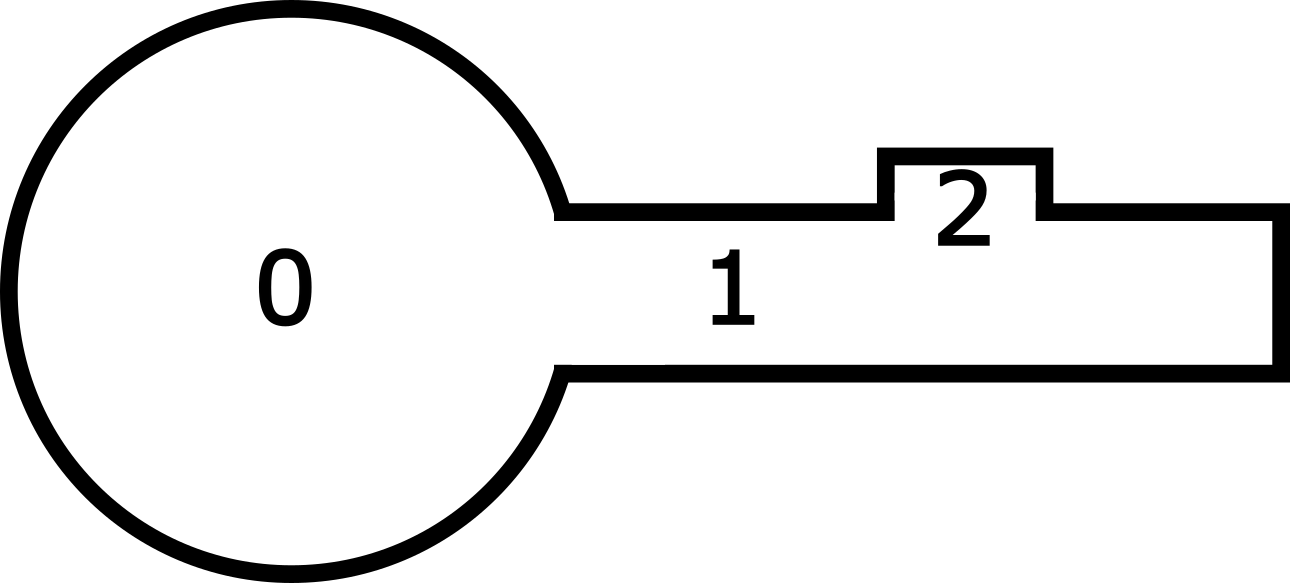
\includegraphics[width=7cm]{img/simplest_neuron.png}
  \end{center}  
  \caption{The simplest (of its kind) model of a neuron with two spatial compartments soma (``$0$'') and unbranched dendrite (``$1$'') with a single synapse (``$2$''). Transcription happens in the soma, while mRNAs and proteins travel between the soma and dendrite degrading over time. Proteins can bind to or unbind from the synapse. Proteins bound to the synapse do not decay. \textcolor{purple}{I will update this figure later to be much bigger and include all the processes as arrows with the corresponding rates.}}
  \label{fig:simplest_neuron}
\end{figure}
In this section we attempt to find the means and the variances of the protein counts in the simplest possible model of neuron of our kind.

\begin{align*}
  &\textcolor{red}{\text{Gene activation:}} \quad &&\textcolor{red}{n_1 \xrightarrow[]{\lambda_1^+(N-n_1)} n_1+1}\\
  &\textcolor{red}{\text{Gene inactivation:}}  &&\textcolor{red}{n_1 \xrightarrow[]{\lambda_1^-n_1} n_1-1}\\
  &\textcolor{green}{\text{Transcription (only in soma):}} &&\textcolor{green}{m_0 \xrightarrow[]{\lambda_2n_1} m_0+1}\\
  &\textcolor{green}{\text{mRNA degradation in $i$-th dendritic compartment:}} &&\textcolor{green}{m_i \xrightarrow[]{m_i/\tau_2} m_i-1}\\
  &\textcolor{blue}{\text{mRNA hopping from dendritic compartment $i$ to $j$:}} &&\textcolor{blue}{(m_i, m_j) \xrightarrow[]{\nu_{ij}m_i} (m_i-1, m_j+1)}\\
  &\textcolor{brown}{\text{Translation (in all nonsynaptic compartments):}} &&\textcolor{brown}{l_i \xrightarrow[]{m_i\kappa_i} l_i+1}\\
  &\textcolor{brown}{\text{Proteolysis in dendritic compartment $i$:}} &&\textcolor{brown}{l_i \xrightarrow[]{l_i/\tau_3} l_i-1}\\
  &\textcolor{cyan}{\text{Protein hopping from dendritic compartment $i$ to $j$:}} &&\textcolor{cyan}{(l_i, l_j) \xrightarrow[]{\theta_{ij}l_i} (l_i-1, l_j+1)}\\
  &\textcolor{violet}{\text{Protein binding to $j$-th synapse on $i$-th compartment:}} &&\textcolor{violet}{(q_{ij}, l_i) \xrightarrow[]{\eta_{ij}l_i} (q_{ij}+1, l_i-1)}\\
  &\textcolor{violet}{\text{Protein unbinding from $j$-th synapse on $i$-th compartment:}} &&\textcolor{violet}{(q_{ij}, l_i) \xrightarrow[]{\gamma_{ij}q_{ij}} (q_{ij}-1, l_i+1)}
\end{align*}

\textcolor{purple}{Note that in this initial formulation we assume that proteins do not decay in synapses (which is easy to change), and, although in these notes the mRNA and protein decay rates are assumed constant throughout the entire neuron, they can be set separately in our software.}% Also, there is no reason other than indexing synapses by pairs of indices (e.g. $j$-th synapse on $i$-th compartment) for considering binding/unbinding of proteins to/from synapses as something other than protein hopping between compartments, so we may change the notation later and get rid of $\eta_{ij}$, $\gamma_{ij}$ and $q_{ij}$.}
  
\subsubsection{Master equation}
The model should capture the following:
\begin{enumerate}
\item \textcolor{red}{Gene activation/deactivation};
\item \textcolor{green}{mRNA production (only in the soma) and degradation (in both compartments)};
\item \textcolor{blue}{mRNA hopping};
\item \textcolor{brown}{Protein production (in both compartments) and degradation (in both compartments, but not in the synapse)};
\item \textcolor{cyan}{Protein hopping};
\item \textcolor{violet}{Protein binding/unbinding from the synapse}.
\end{enumerate}
The master equation that captures these processes reads as
\begin{equation*}
  \begin{split}
    \frac{dP_{\mathbf s}(t)}{dt} &= \textcolor{red}{\lambda_1^+\left[\left(N-n+1\right)P_{n-1}^{\mathbf s}(t) - \left(N-n\right)P_{\mathbf s}(t)\right] + \lambda_1^-\left[(n+1)P^{\mathbf s}_{n+1}(t) - nP_{\mathbf s}(t)\right]}\\
    & \textcolor{green}{+ \lambda_2n\left[P^{\mathbf s}_{m_0-1}(t) - P_{\mathbf s}(t)\right] + \frac{1}{\tau_2}\left[(m_0+1)P^{\mathbf s}_{m_0+1}(t) - m_0P_{\mathbf s}(t)\right]}\\ &\textcolor{green}{+ \frac{1}{\tau_2}\left[(m_1+1)P^{\mathbf s}_{m_1+1}(t) - m_1P_{\mathbf s}(t)\right]} \textcolor{blue}{+ \nu_{01}\left[(m_0+1)P^{\mathbf s}_{m_0+1,m_1-1}(t) - m_0P_{\mathbf s}(t)\right]}\\
    &\textcolor{blue}{+ \nu_{10}\left[(m_1+1)P^{\mathbf s}_{m_0-1,m_1+1}(t) - m_1P_{\mathbf s}(t)\right]} \textcolor{brown}{+ \kappa_0m_0\left[P^{\mathbf s}_{l_0-1}(t) - P_{\mathbf s}(t)\right]}\\
    &\textcolor{brown}{+ \kappa_1m_1\left[P^{\mathbf s}_{l_1-1}(t) - P_{\mathbf s}(t)\right] + \frac{1}{\tau_3}\left[(l_0+1)P^{\mathbf s}_{l_0+1}(t) - l_0P_{\mathbf s}(t)\right]}\\&\textcolor{brown}{+ \frac{1}{\tau_3}\left[(l_1+1)P^{\mathbf s}_{l_1+1}(t)-l_1P_{\mathbf s}(t)\right]} \textcolor{cyan}{+ \theta_{01}\left[(l_0+1)P^{\mathbf s}_{l_0+1,l_1-1}(t) - l_0P_{\mathbf s}(t)\right]}\\
    &\textcolor{cyan}{+ \theta_{10}\left[(l_1+1)P^{\mathbf s}_{l_0-1,l_1+1}(t) - l_1P_{\mathbf s}(t)\right]} \textcolor{violet}{+\eta_{11}\left[(l_1+1)P^{\mathbf s}_{l_1+1, q_{11}-1}(t) - l_1P_{\mathbf s}(t)\right]} \\
    &\textcolor{violet}{+ \gamma_{11}\left[(q_{11}+1)P^{\mathbf s}_{l_1-1,q_{11}+1}(t) - q_{11}P_{\mathbf s}(t)\right]}.
  \end{split}
\end{equation*}

\subsubsection{PDE for the generating function}
\begin{equation*}
  \begin{split}
    & \frac{\partial\mathcal G(\mathbf x; t)}{\partial t} + \left(\lambda^+_1x_n^2-\lambda_2x_{m_0}x_n + \frac{1}{\tau_1}x_n - \lambda_2x_{m_0}\right)\frac{\partial\mathcal G(\mathbf x; t)}{\partial x_n}\\
    &- \left[\kappa_0x_{m_0}x_{l_0} + \kappa_0x_{l_0} + \nu_{01}x_{m_1} - \left(\frac{1}{\tau_2}+\nu_{01}\right)x_{m_0}\right]\frac{\partial \mathcal G(\mathbf x; t)}{\partial x_{m_0}}\\ & -\left[\kappa_1x_{m_1}x_{l_1} + \kappa_1x_{l_1} + \nu_{10}x_{m_0} - \left(\nu_{10}+\frac{1}{\tau_2}\right)x_{m_1}\right]\frac{\partial\mathcal G(\mathbf x; t)}{\partial x_{m_1}}\\
    &+\left[\left(\frac{1}{\tau_3}+\theta_{01}\right)x_{l_0} - \theta_{01}x_{l_1}\right]\frac{\partial\mathcal G(\mathbf x; t)}{\partial x_{l_0}}\\
    & + \left[\left(\frac{1}{\tau_3} + \theta_{10} + \eta_{11}\right)x_{l_1} - \theta_{10}x_{l_0} -\eta_{11}x_{q_{11}}\right]\frac{\partial\mathcal G(\mathbf x; t)}{\partial x_{l_1}}\\
    &+\gamma_{11}(x_{q_{11}} - x_{l_1})\frac{\partial\mathcal G(\mathbf x; t)}{\partial x_{q_{11}}} = \lambda_1^+x_nN\mathcal G(\mathbf x; t)
  \end{split}
\end{equation*}

%% Renaming
%% \begin{equation}
%%   (x_n, x_{m_0}, x_{m_1}, x_{l_0}, x_{l_1}, x_{q_{11}}) \equiv (x_1, x_2, x_3, x_4, x_5, x_6)
%% \end{equation}

First order:
\begin{align*}
  \mathcal G_1 &= \tau_1\lambda_1^+N\\
  \mathcal G_2 &= \frac{\lambda_2\tau_2(\tau_2\nu_{10}+1)}{\tau_2(\nu_{01}+\nu_{10})+1}\tau_1\lambda_1^+N\\
  \mathcal G_3 &= \frac{\lambda_2\tau_2^2\nu_{01}}{\tau_2(\nu_{01}+\nu_{10})+1}\tau_1\lambda_1^+N\\
  \mathcal G_4 &= \frac{\kappa_0(\nu_{10}\tau_2+1)(\tau_3\theta_{10}+1) + \kappa_1\nu_{01}\tau_2\tau_3\theta_{10}}{\left[\tau_2(\nu_{01}+\nu_{10})+1\right]\left[\tau_3(\theta_{01}+\theta_{10})+1\right]}\tau_3\lambda_2\tau_2\lambda_1^+\tau_1N\\
  \begin{split}
    \mathcal G_5 &= \frac{\kappa_1\nu_{01}\tau_2\left[\tau_3(\theta_{01}+\theta_{10})+1\right] + \tau_3\theta_{01}\left[\kappa_0(\nu_{10}\tau_2+1)(\tau_3\theta_{10}+1) + \kappa_1\nu_{01}\tau_2\tau_3\theta_{10}\right]}{\left[\tau_2(\nu_{01}+\nu_{10})+1\right]\left(\tau_3\theta_{10}+1\right)\left[\tau_3(\theta_{01}+\theta_{10})+1\right]}\tau_3\lambda_2\tau_2\lambda_1^+\tau_1N\\
    &=\left[\kappa_1\nu_{01}\tau_2 + \frac{\tau_3\theta_{01}\left[\kappa_0(\nu_{10}\tau_2+1)(\tau_3\theta_{10}+1)+\kappa_1\nu_{01}\tau_2\tau_3\theta_{10}\right]}{\tau_3(\theta_{01}+\theta_{10})+1}\right]\frac{\tau_3\lambda_2\tau_2\lambda_1^+\tau_1N}{\left[\tau_2(\nu_{01}+\nu_{10})+1\right](\tau_3\theta_{10}+1)}
  \end{split}\\
  \begin{split}
    \mathcal G_6 &= \frac{\eta_{11}}{\gamma_{11}}\frac{\kappa_1\nu_{01}\tau_2\left[\tau_3(\theta_{01}+\theta_{10})+1\right] + \tau_3\theta_{01}\left[\kappa_0(\nu_{10}\tau_2+1)(\tau_3\theta_{10}+1) + \kappa_1\nu_{01}\tau_2\tau_3\theta_{10}\right]}{\left[\tau_2(\nu_{01}+\nu_{10})+1\right]\left(\tau_3\theta_{10}+1\right)\left[\tau_3(\theta_{01}+\theta_{10})+1\right]}\tau_3\lambda_2\tau_2\lambda_1^+\tau_1N\\
    &= \left[\kappa_1\nu_{01}\tau_2 + \frac{\tau_3\theta_{01}\left[\kappa_0(\nu_{10}\tau_2+1)(\tau_3\theta_{10}+1)+\kappa_1\nu_{01}\tau_2\tau_3\theta_{10}\right]}{\tau_3(\theta_{01}+\theta_{10})+1}\right]\frac{\eta_{11}\tau_3\lambda_2\tau_2\lambda_1^+\tau_1N}{\gamma_{11}\left[\tau_2(\nu_{01}+\nu_{10})+1\right](\tau_3\theta_{10}+1)}
  \end{split}
\end{align*}

Second-order expressions are not shown here due to their size, but they are obtained using symbolic computing software.

\subsection{Simple neuron model}
\subsubsection{PDE for the generating function}
\begin{equation*}
  \begin{split}
    & \frac{\partial\mathcal G(\mathbf x; t)}{\partial t} + \left(\lambda^+_1x_n^2-\lambda_2x_{m_0}x_n + \frac{1}{\tau_1}x_n - \lambda_2x_{m_0}\right)\frac{\partial\mathcal G(\mathbf x; t)}{\partial x_n}\\
    &+\left[-\kappa_0x_{m_0}x_{l_0} + \left(\frac{1}{\tau_2}+\nu_{01}\right)x_{m_0} - \kappa_0x_{l_0} - \nu_{01}x_{m_1}\right]\frac{\partial \mathcal G(\mathbf x; t)}{\partial x_{m_0}}\\
    &+\left[- \kappa_1x_{m_1}x_{l_1} +\left(\nu_{10}+\nu_{12}+\nu_{13}+\frac{1}{\tau_2}\right)x_{m_1} - \kappa_1x_{l_1} - \nu_{10}x_{m_0}  - \nu_{12}x_{m_2} - \nu_{13}x_{m_3}\right]\frac{\partial\mathcal G(\mathbf x; t)}{\partial x_{m_1}}\\
    &+\left[-\kappa_2x_{m_2}x_{l_2} - \kappa_2x_{l_2} - \nu_{21}x_{m_1} + \left(\nu_{21} + \frac{1}{\tau_2}\right)x_{m_2}\right]\frac{\partial\mathcal G(\mathbf x; t)}{\partial x_{m_2}}\\
    &+\left[-\kappa_3x_{m_3}x_{l_3} - \kappa_3x_{l_3} - \nu_{31}x_{m_1} + \left(\nu_{31} + \frac{1}{\tau_2}\right)x_{m_3}\right]\frac{\partial\mathcal G(\mathbf x; t)}{\partial x_{m_3}}\\
    &+\left[\left(\frac{1}{\tau_3}+\theta_{01}\right)x_{l_0} - \theta_{01}x_{l_1}\right]\frac{\partial\mathcal G(\mathbf x; t)}{\partial x_{l_0}}\\ %THIS IS STRANGE BECAUSE THERE IS A FLOW OF PROTEINS FROM THE MAIN DENDRITE
    &+\left[\left(\eta_{11}+\eta_{12}+\theta_{10}+\theta_{12}+\theta_{13}+\frac{1}{\tau_3}\right)x_{l_1} - \eta_{11}x_{q_{11}} - \eta_{12}x_{q_{12}} - \theta_{10}x_{l_0} - \theta_{12}x_{l_2} - \theta_{13}x_{l_3}\right]\frac{\partial\mathcal G(\mathbf x; t)}{\partial x_{l_1}}\\
    &+\left[\left(\eta_{21}+\eta_{22}+\theta_{21}+\frac{1}{\tau_3}\right)x_{l_2} - \eta_{21}x_{q_{21}} - \eta_{22}x_{q_{22}} - \theta_{21}x_{l_1}\right]\frac{\partial\mathcal G(\mathbf x;t)}{\partial x_{l_2}}\\ 
    &+\left[\left(\eta_{31}+\eta_{32}+\theta_{31}+\frac{1}{\tau_3}\right)x_{l_3} - \eta_{31}x_{q_{31}} - \eta_{32}x_{q_{32}} - \theta_{31}x_{l_1} \right]\frac{\partial\mathcal G(\mathbf x;t)}{\partial x_{l_3}}\\ 
    &+\gamma_{11}\left(x_{q_{11}}-x_{l_1}\right)\frac{\partial\mathcal G(\mathbf x;t)}{\partial x_{q_{11}}} + \gamma_{12}\left(x_{q_{12}}-x_{l_1}\right)\frac{\partial\mathcal G(\mathbf x;t)}{\partial x_{q_{12}}}\\
    &+\gamma_{21}\left(x_{q_{21}}-x_{l_2}\right)\frac{\partial\mathcal G(\mathbf x;t)}{\partial x_{q_{21}}} + \gamma_{22}\left(x_{q_{22}}-x_{l_2}\right)\frac{\partial\mathcal G(\mathbf x;t)}{\partial x_{q_{22}}}\\
    &+\gamma_{31}\left(x_{q_{31}}-x_{l_3}\right)\frac{\partial\mathcal G(\mathbf x;t)}{\partial x_{q_{31}}} + \gamma_{32}\left(x_{q_{32}}-x_{l_3}\right)\frac{\partial\mathcal G(\mathbf x;t)}{\partial x_{q_{32}}}\\
    &=\lambda_1^+x_nN\mathcal G(\mathbf x; t)
  \end{split}
\end{equation*}

\subsubsection{Numeric results}
In Table \ref{table:expectations_errors} are the expectations, fluctuations and noise to signal ratios.
%% \begin{center}
%% \begin{tabular}{ |c|c| } 
%%   \hline
%%   $\langle n\rangle$ & $1$\\                 \hline
%%   $\langle m_0\rangle$  & $1.79590072201514$\\  \hline
%%   $\langle m_1\rangle$  & $1.2981274878913$S\\   \hline
%%   $\langle m_2\rangle$  & $0.952985895047784$\\ \hline
%%   $\langle m_3\rangle$  & $0.952985895046793$\\ \hline
%%   $\langle l_0\rangle$  & $28966.7621095089$\\  \hline
%%   $\langle l_1\rangle$  & $28522.7399412071$\\  \hline
%%   $\langle l_2\rangle$  & $14643.6787267151$\\  \hline
%%   $\langle l_3\rangle$  & $14643.6787267138$\\  \hline
%%   $\langle q_{11}\rangle$  & $2852.27399412071$\\  \hline
%%   $\langle q_{12}\rangle$  & $2852.27399412071$\\  \hline
%%   $\langle q_{21}\rangle$  & $1464.36787267151$\\  \hline
%%   $\langle q_{22}\rangle$  & $1464.36787267151$\\  \hline
%%   $\langle q_{31}\rangle$  & $1464.36787267138$\\  \hline
%%   $\langle q_{32}\rangle$  & $1464.36787267138$\\
%%  \hline
%% \end{tabular}
%% \end{center}

\begin{table}
  \begin{center}
    \begin{tabular}{ |c|c|c|c| }
      \hline
      Variable &Expectation          & $\sigma$    & $\sigma$/Expectation\%\\  \hline
      $n$      & $1$                 & $0$    & $0$ \\                 \hline
      $m_0$    & $1.79590072201514$  & $1.3401122038414643$ & $74.6206172431264$\\  \hline
      $m_1$    & $1.2981274878913$   & $1.139353975003979$ & $87.7690354477251$\\   \hline
      $m_2$    & $0.952985895047784$ & $0.9762099620737184$ & $102.436979093460$\\ \hline
      $m_3$    & $0.952985895046793$ & $0.9762099634821508$ & $102.436979241358$\\ \hline
      $l_0$    & $28966.7621095089$  & $3600.673144730757$ & $12.4303611536505$\\  \hline
      $l_1$    & $28522.7399412071$  & $3640.7733140368373$ & $12.7644585391917$\\  \hline
      $l_2$    & $14643.6787267151$  & $2356.5543166178854$ & $16.0926387460190$\\  \hline
      $l_3$    & $14643.6787267138$  & $2356.5543207336664$ & $16.0926387741265$\\  \hline
      $q_{11}$ & $2852.27399412071$  & $367.58407810640534$ & $12.8874041857162$\\  \hline
      $q_{12}$ & $2852.27399412071$  & $367.5840781064142$ & $12.8874041857165$\\  \hline
      $q_{21}$ & $1464.36787267151$  & $238.43365659083406$ & $16.2823605352560$\\  \hline
      $q_{22}$ & $1464.36787267151$  & $238.433656590837$ & $16.2823605352562$ \\  \hline
      $q_{31}$ & $1464.36787267138$  & $238.433656997613$ & $16.2823605630359$ \\  \hline
      $q_{32}$ & $1464.36787267138$ & $238.43365699761108$ & $16.2823605630358$ \\
      \hline
    \end{tabular}
    \caption{\label{table:expectations_errors}Expectations, noise and noise to signal ratios. Note that, in this setting, variances of mRNA distributions are identical to their means, which suggests their Poissonian nature. This, presumably, should not be the case if the gene in not assumed to be always active.}
  \end{center}
\end{table}


%% \begin{center}
%%   \begin{tabular}{ |c|c| }
%%     \hline
%%     Variable & RMS$(.)/\langle .\rangle\cdot100\%$\\  \hline
%%     $n$     & $0$\\                 \hline
%%     $m_0$   & $74.6206172431264$\\  \hline
%%     $m_1$   & $87.7690354477251$\\   \hline
%%     $m_2$   & $102.436979093460$\\ \hline
%%     $m_3$   & $102.436979241358$\\ \hline
%%     $l_0$   & $12.4303611536505$\\  \hline
%%     $l_1$   & $12.7644585391917$\\  \hline
%%     $l_2$   & $16.0926387460190$\\  \hline
%%     $l_3$   & $16.0926387741265$\\  \hline
%%     $q_{11}$ & $12.8874041857162$\\  \hline
%%     $q_{12}$ & $12.8874041857165$\\  \hline
%%     $q_{21}$ & $16.2823605352560$\\  \hline
%%     $q_{22}$ & $16.2823605352562$\\  \hline
%%     $q_{31}$ & $16.2823605630359$\\  \hline
%%     $q_{32}$ & $16.2823605630358$\\
%%     \hline
%%   \end{tabular}
%% \end{center}


\subsection{General rules}
This section provides the general rules for constructing a {\it master equation} and the corresponding PDE for the generating function from the neuron's compartments diagram analogous to the one in Figure \ref{fig:simplest_neuron}. For this reason we represent a neuron as a graph which nodes represent different compartments of the neuron and the edges represent the junctions between the compartments.

\subsubsection{The rules}
              {\bf Soma}
              
              {\it Parameters:}
              \begin{equation*}
                \{\lambda_1^+, \lambda_1^-, \lambda_2, \tau_2, \tau_3, \kappa_0, N\}
              \end{equation*}

              {\it Variables:}
              \begin{equation*}
                \{n, m_0, l_0\}\ \ \ \left(\{x_n, x_{m_0}, x_{l_0}\}\text{ in the PDE}\right)
              \end{equation*}

              
              {\it ME terms:}
              \begin{equation}
                \begin{split}
                  &\textcolor{red}{\lambda_1^+\left[\left(N-n+1\right)P_{n-1}^{\mathbf s}(t) - \left(N-n\right)P_{\mathbf s}(t)\right] + \lambda_1^-\left[(n+1)P^{\mathbf s}_{n+1}(t) - nP_{\mathbf s}(t)\right]}\\
                  &\textcolor{green}{+ \lambda_2n\left[P^{\mathbf s}_{m_0-1}(t) - P_{\mathbf s}(t)\right] + \frac{1}{\tau_2}\left[(m_0+1)P^{\mathbf s}_{m_0+1}(t) - m_0P_{\mathbf s}(t)\right]}\\
                  &\textcolor{brown}{+ \kappa_0m_0\left[P^{\mathbf s}_{l_0-1}(t) - P_{\mathbf s}(t)\right] + \frac{1}{\tau_3}\left[(l_0+1)P^{\mathbf s}_{l_0+1}(t) - l_0P_{\mathbf s}(t)\right]}
                \end{split}
              \end{equation}
              
              {\it Corresponding PDE terms\footnote{Should be understood as $\frac{\partial\mathcal G}{\partial t} =$ (Sum of these PDE terms).}:}
              \begin{equation}
                \begin{split}
                  \lambda_1^+x_nN\mathcal G(\mathbf x, t)
                  - \left[\lambda_1^+x_n^2 - \lambda_2x_{m_0}x_n + (\lambda_1^++\lambda_1^-)x_n-\lambda_2x_{m_0}\right]\frac{\partial\mathcal G(\mathbf x, t)}{\partial x_n}\\
                  - \left[-\kappa_0x_{m_0}x_{l_0} - \kappa_0x_{l_0} + \frac{1}{\tau_2}x_{m_0}\right]\frac{\partial\mathcal G(\mathbf x, t)}{\partial x_{m_0}}
                  -\frac{1}{\tau_3}x_{l_0}\frac{\partial\mathcal G(\mathbf x, t)}{\partial x_{l_0}}
                \end{split}
              \end{equation}


              {\bf Dendritic compartment}
              
              {\it Parameters:}
              \begin{equation*}
                \{\tau_2, \kappa_i, \tau_3\}
              \end{equation*}

              {\it Variables:}
              \begin{equation*}
                \{m_i, l_i\}\ \ \ \left(\{x_{m_i}, x_{l_i}\}\text{ in the PDE}\right)
              \end{equation*}

              
              {\it ME terms:}
              \begin{equation}
                \begin{split}
                  \textcolor{green}{\frac{1}{\tau_2}\left[(m_i+1)P_{m_i+1}^{\mathbf s}(t) - m_iP_{\mathbf s}(t)\right]} \textcolor{brown}{+ \kappa_im_i\left[P_{l_i-1}^{\mathbf s}(t) - P_{\mathbf s}(t)\right]}\\
                  \textcolor{brown}{+ \frac{1}{\tau_3}\left[(l_i+1)P_{l_i+1}^{\mathbf s}(t) - l_iP_{\mathbf s}(t)\right]}
                \end{split}
              \end{equation}
              
              {\it Corresponding PDE terms:}
              \begin{equation}
                \begin{split}
                  -\left[-\kappa_ix_{m_i}x_{l_i} - \kappa_ix_{l_i} + \frac{1}{\tau_2}x_{m_i}\right]\frac{\partial \mathcal G(\mathbf x, t)}{\partial x_{m_i}} - \frac{1}{\tau_3}x_{l_i}\frac{\partial\mathcal G(\mathbf x, t)}{\partial x_{l_i}}
                \end{split}
              \end{equation}


              {\bf Synapse $j$ on dendrite $i$}

              {\it Parameters:}
              \begin{equation*}
                \text{\footnotesize{Could be protein decay/production rates, mRNA decay or something else, but empty for now.}}
              \end{equation*}

              {\it Variables:}
              \begin{equation*}
                q_{ij}
              \end{equation*}

              
              {\it ME terms:}
              \begin{equation}
                \emptyset
              \end{equation}
              
              {\it Corresponding PDE terms:}
              \begin{equation}
                \emptyset
              \end{equation}


              {\bf Junction between two non-synaptic compartments}
              
              {\it Parameters:}
              \begin{equation*}
                \{\nu_{ij}, \nu_{ji}, \theta_{ij}, \theta_{ji}\}
              \end{equation*}

              {\it Variables:}
              \begin{equation*}
                \emptyset
              \end{equation*}

              
              {\it ME terms:}
              \begin{equation}
                \begin{split}
                  \textcolor{blue}{\nu_{ij}\left[(m_i+1)P_{m_i+1, m_j-1}^{\mathbf s}(t) - m_iP_{\mathbf s}(t)\right] + \nu_{ji}\left[(m_j+1)P_{m_i-1, m_j+1}^{\mathbf s}(t) - m_jP_{\mathbf s}(t)\right]}\\
                  \textcolor{cyan}{+ \theta_{ij}\left[(l_i+1)P_{l_i+1, l_j-1}^{\mathbf s}(t) - l_iP_{\mathbf s}(t)\right] + \theta_{ji}\left[(l_j+1)P_{l_i-1, l_j+1}^{\mathbf s}(t) - l_jP_{\mathbf s}(t)\right]}
                \end{split}
              \end{equation}
              
              {\it Corresponding PDE terms:}
              \begin{equation}
                \begin{split}
                  -\nu_{ij}(x_{m_i}-x_{m_j})\frac{\partial\mathcal G(\mathbf x, t)}{\partial x_{m_i}} - \nu_{ji}(x_{m_j}-x_{m_i})\frac{\partial\mathcal G(\mathbf x, t)}{\partial x_{m_j}}\\
                  -\theta_{ij}(x_{l_i}-x_{l_j})\frac{\partial\mathcal G(\mathbf x, t)}{\partial x_{l_i}} - \theta_{ji}(x_{l_j}-x_{l_i})\frac{\partial\mathcal G(\mathbf x, t)}{\partial x_{l_j}}
                \end{split}
              \end{equation}

              {\bf Junction between the dendrite i and the synapse j on it}
              
              {\it Parameters:}
              \begin{equation*}
                \{\eta_{ij}, \gamma_{ij}\}
              \end{equation*}

              {\it Variables:}
              \begin{equation*}
                \emptyset
              \end{equation*}

              {\it ME terms:}
              \begin{equation}
                \begin{split}
                  \textcolor{violet}{\eta_{ij}\left[(l_i+1)P_{l_i+1, q_{ij}-1}^{\mathbf s}(t) - l_iP_{\mathbf s}(t)\right] + \gamma_{ij}\left[(q_{ij}+1)P_{l_i-1, q_{ij}+1}^{\mathbf s}(t) - q_{ij}P_{\mathbf s}(t)\right]}
                \end{split}
              \end{equation}
              
              {\it Corresponding PDE terms:}
              \begin{equation}
                -\eta_{ij}(x_{l_i}-x_{q_{ij}})\frac{\partial\mathcal G(\mathbf x, t)}{\partial x_{l_i}} - \gamma_{ji}(x_{q_{ij}}-x_{l_i})\frac{\partial\mathcal G(\mathbf x, t)}{\partial x_{q_{ij}}}
              \end{equation}
              
              \subsubsection{Second-order expansions}
              When substituted to the above PDE terms corresponding to the compartments of certain types, the expansion (\ref{eqn:basic_expansion}) gives the following terms in the second order.
              
              {\bf Soma}
              \begin{multline*}
                \textcolor{blue}{\lambda_1^+Nx_n\boldsymbol{\mathcal G}^{(1)}\mathbf x + \kappa_0x_{m_0}x_{l_0}\mathcal G^{(1)}_{m_0} - \left(\lambda_1^+x_n^2-\lambda_2x_{m_0}x_n\right)\mathcal G_n^{(1)}}\\
                -\left[\left(\lambda_1^++\lambda_1^-\right)x_n-\lambda_2x_{m_0}\right]\boldsymbol{\mathcal G}_n^{(2)}\mathbf x + \left(\kappa_0x_{l_0}-\frac{1}{\tau_2}x_{m_0}\right)\boldsymbol{\mathcal G}_{m_0}^{(2)}\mathbf x - \frac{1}{\tau_3}x_{l_0}\boldsymbol{\mathcal G}^{(2)}_{l_0}\mathbf x
              \end{multline*}
              
              {\bf Dendritic compartment}
              \begin{equation*}
                \textcolor{blue}{\kappa_ix_{m_i}x_{l_i}\mathcal G^{(1)}_{m_i}} + \left(\kappa_ix_{l_i} - \frac{1}{\tau_2}x_{m_i}\right)\boldsymbol{\mathcal G}^{(2)}_{m_i}\mathbf x - \frac{1}{\tau_3}x_{l_i}\boldsymbol{\mathcal G}^{(2)}_{l_i}\mathbf x
              \end{equation*}

              {\bf Junction between two non-synaptic compartments}
              \begin{align*}
                -\nu_{ij}\left(x_{m_i} - x_{m_j}\right)\boldsymbol{\mathcal G}_{m_i}^{(2)}\mathbf x& - \nu_{ji}\left(x_{m_j} - x_{m_i}\right)\boldsymbol{\mathcal G}_{m_j}^{(2)}\mathbf x\\
                - \theta_{ij}\left(x_{l_i}-x_{l_j}\right)\boldsymbol{\mathcal G}_{l_i}^{(2)}\mathbf x& - \theta_{ji}\left(x_{l_j} - x_{l_i}\right)\boldsymbol{\mathcal G}^{(2)}_{l_j}\mathbf x
              \end{align*}

              {\bf Junction between dendrite $i$ and synapse $j$}
              \begin{equation*}
                -\eta_{ij}\left(x_{l_i}-x_{q_{ij}}\right)\boldsymbol{\mathcal G}^{(2)}_{l_i}\mathbf x - \gamma_{ji}\left(x_{q_{ij}}-x_{l_i}\right)\boldsymbol{\mathcal G}^{(2)}_{q_{ij}}\mathbf x
              \end{equation*}

              Note that the terms shown in \textcolor{blue}{blue} are obtained from solving the first-order problem and play the role of a ``source'' in the second-order problem for covariances.

              


\section{Preliminary numerical results}
Some preliminary results for stationary problem are shown in Figs.\ref{fig:3_branching_points_numbers},\ref{fig:10_forks_combined},\ref{10_forks_decay_plots},\ref{fig:linear_model_decays},\ref{fig:4_forks_noise},\ref{fig:4_forks_pearson_correlations}.
\begin{figure}
  \begin{center}
    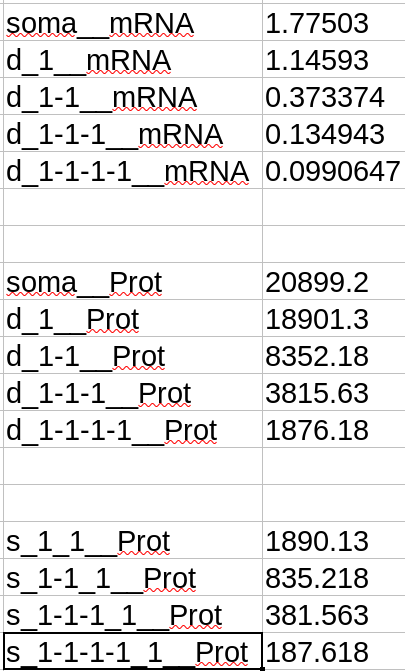
\includegraphics[width=7cm]{img/3_branching_points_numbers.png}
  \end{center}  
  \caption{Protein and mRNA counts' stationary expectations in symmetric model similar to the simple model (same parameters and two synapses on every dendritic segment), but with {\bf three} branching points in each full path up the dendritic tree.}
  \label{fig:3_branching_points_numbers}
\end{figure}

\begin{figure}
  \begin{center}
    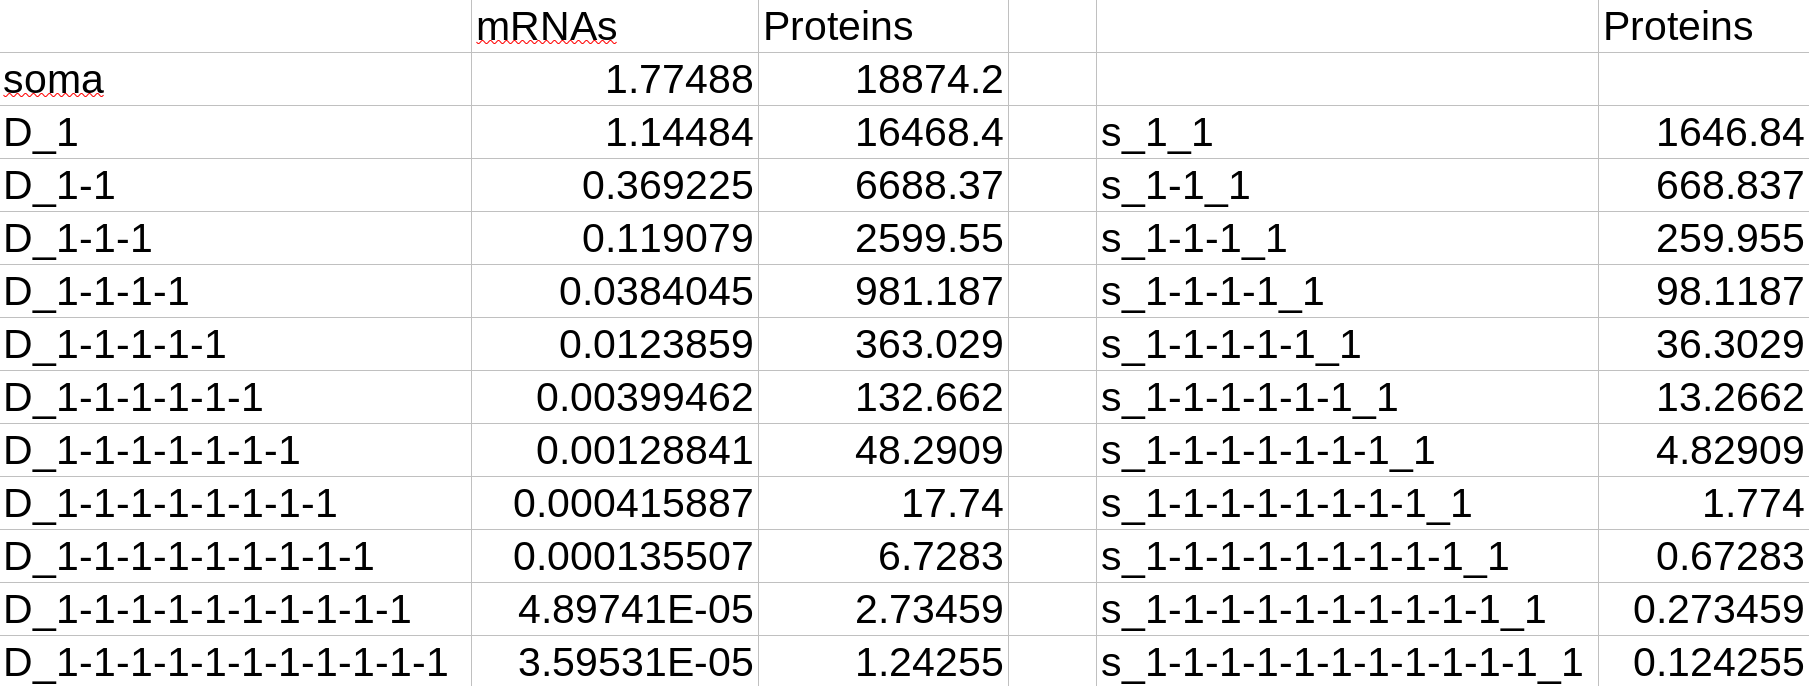
\includegraphics[width=12cm]{img/10_forks_combined.png}
  \end{center}  
  \caption{Protein and mRNA counts in symmetric model similar to the simple model (same parameters and two synapses on every dendritic segment), but with {\bf ten} branching points in each full path up the dendritic tree.}
  \label{fig:10_forks_combined}
\end{figure}

\begin{figure}
  \begin{center}
    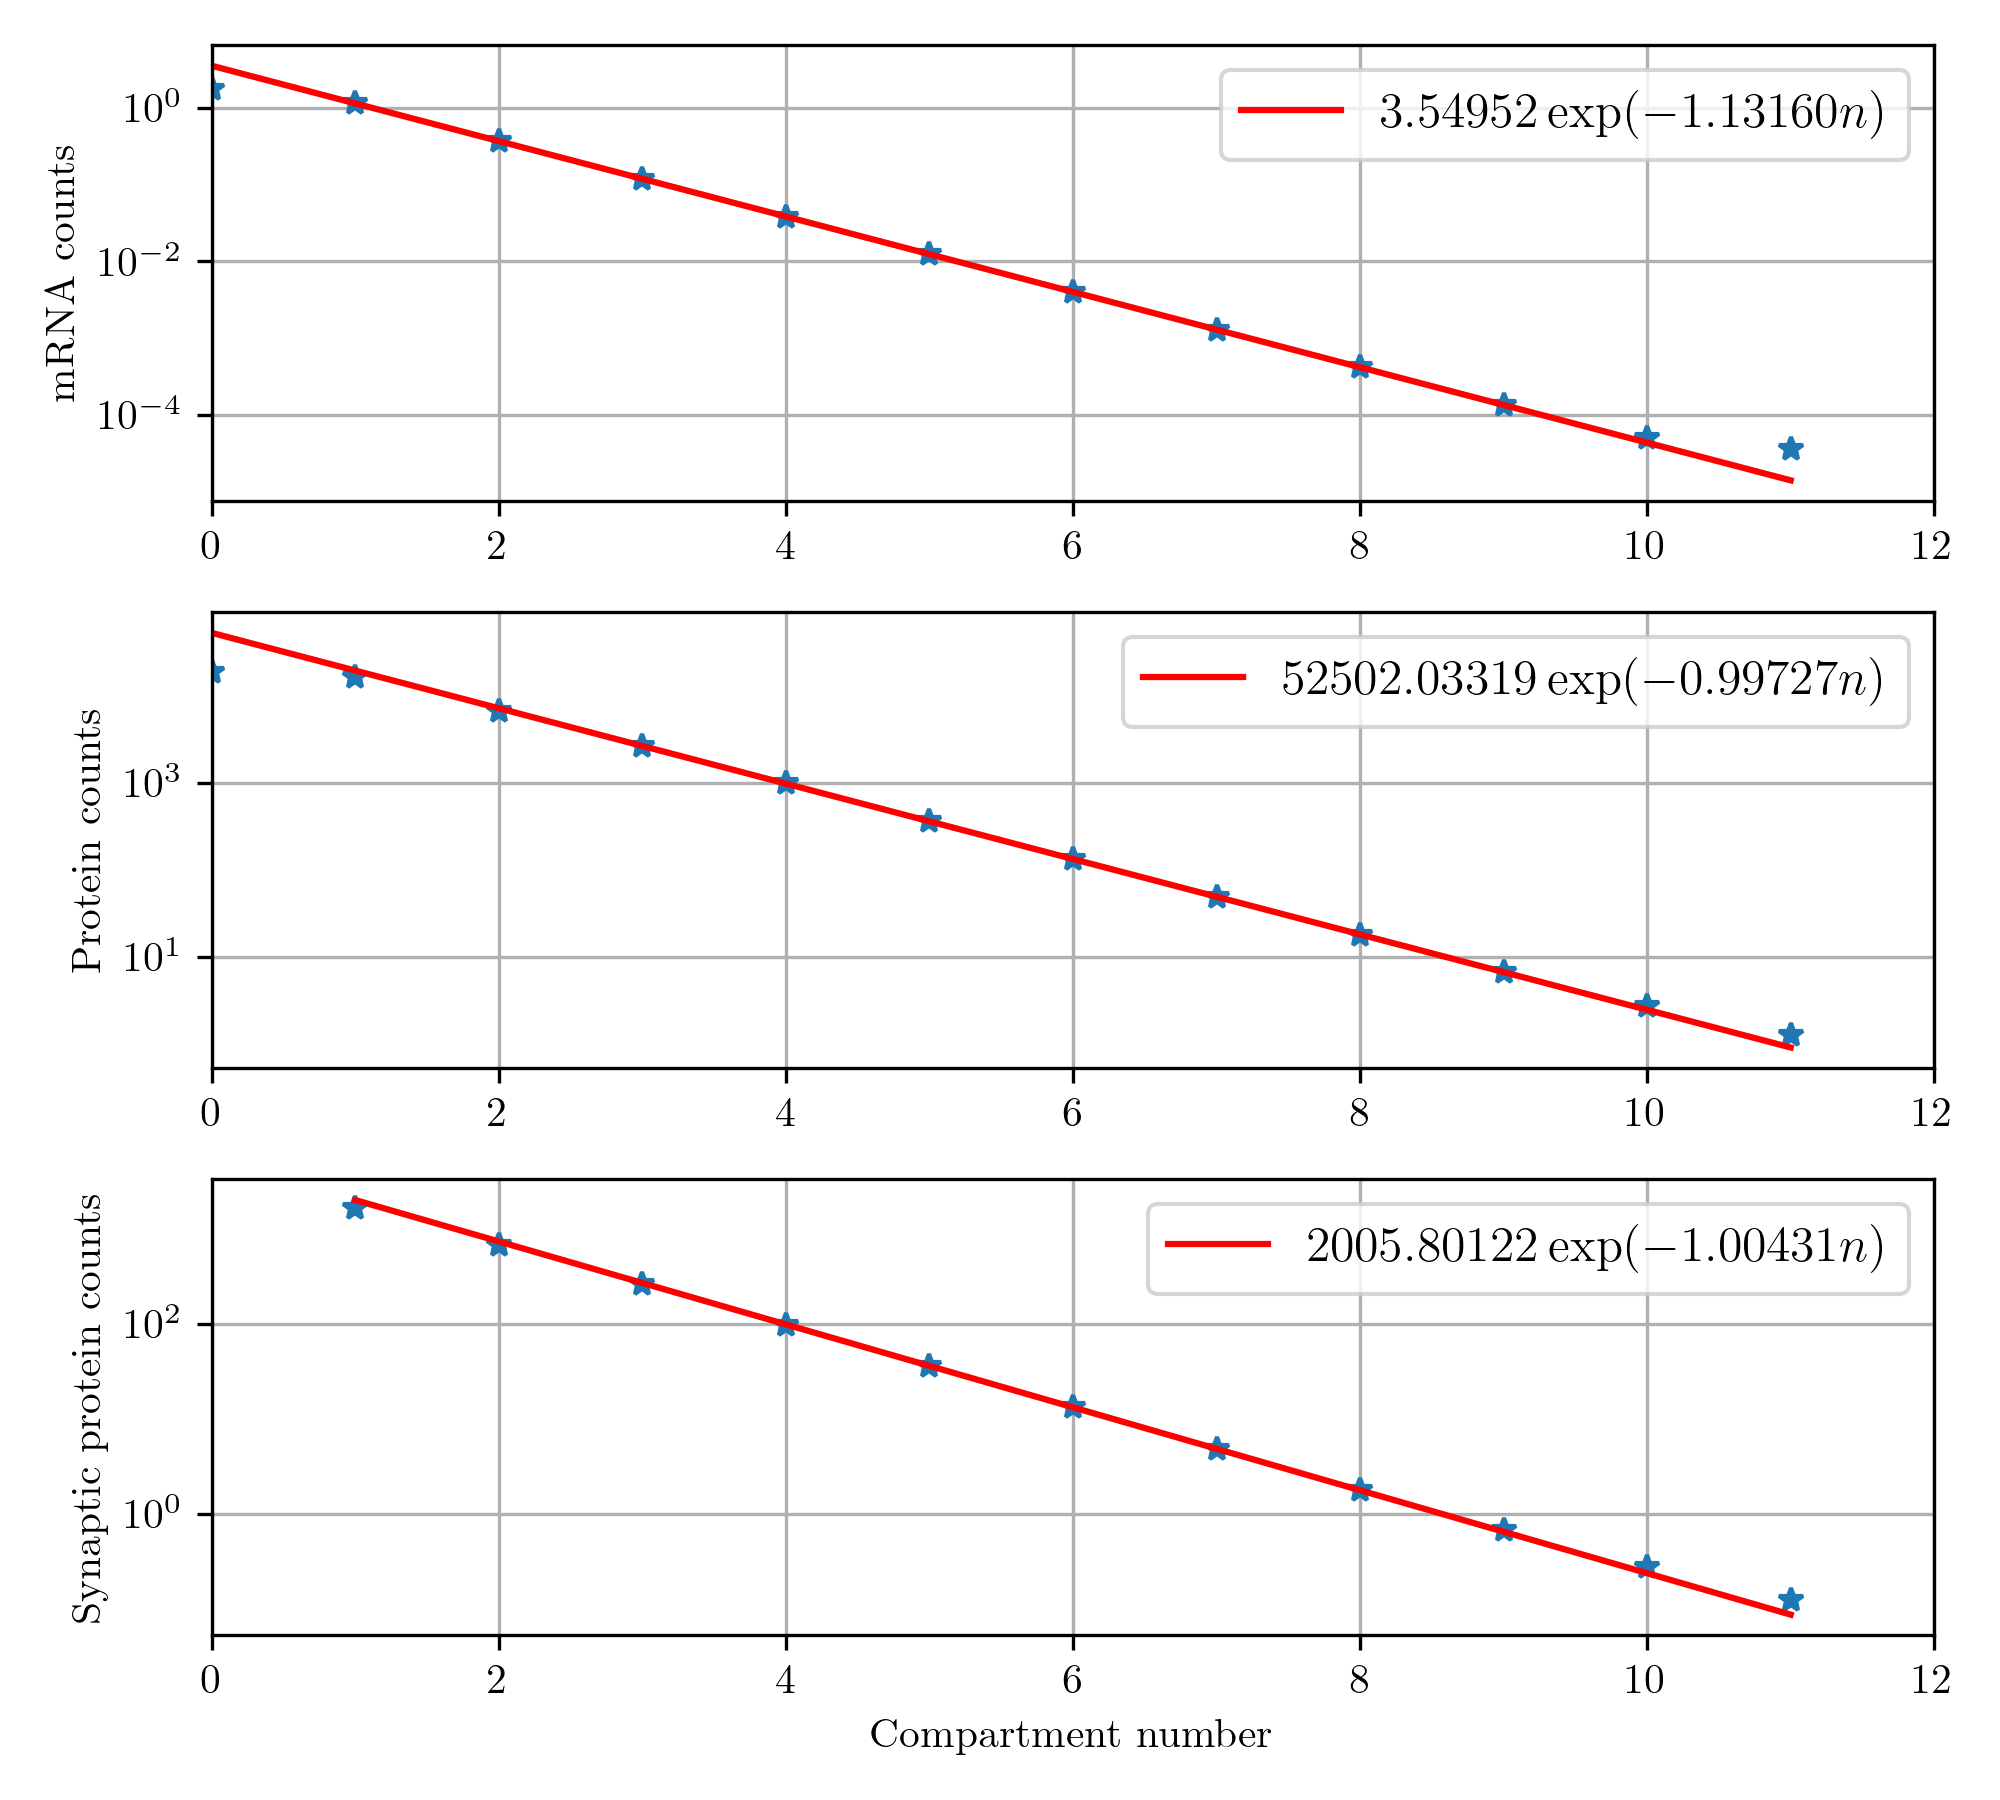
\includegraphics[width=12cm]{img/10_forks_decay_plots.png}
  \end{center}  
  \caption{Protein and mRNA counts in symmetric model similar to the simple model (same parameters and two synapses on every dendritic segment), but with {\bf ten} branching points in each full path up the dendritic tree.}
  \label{10_forks_decay_plots}
\end{figure}

\begin{figure}
  \begin{center}
    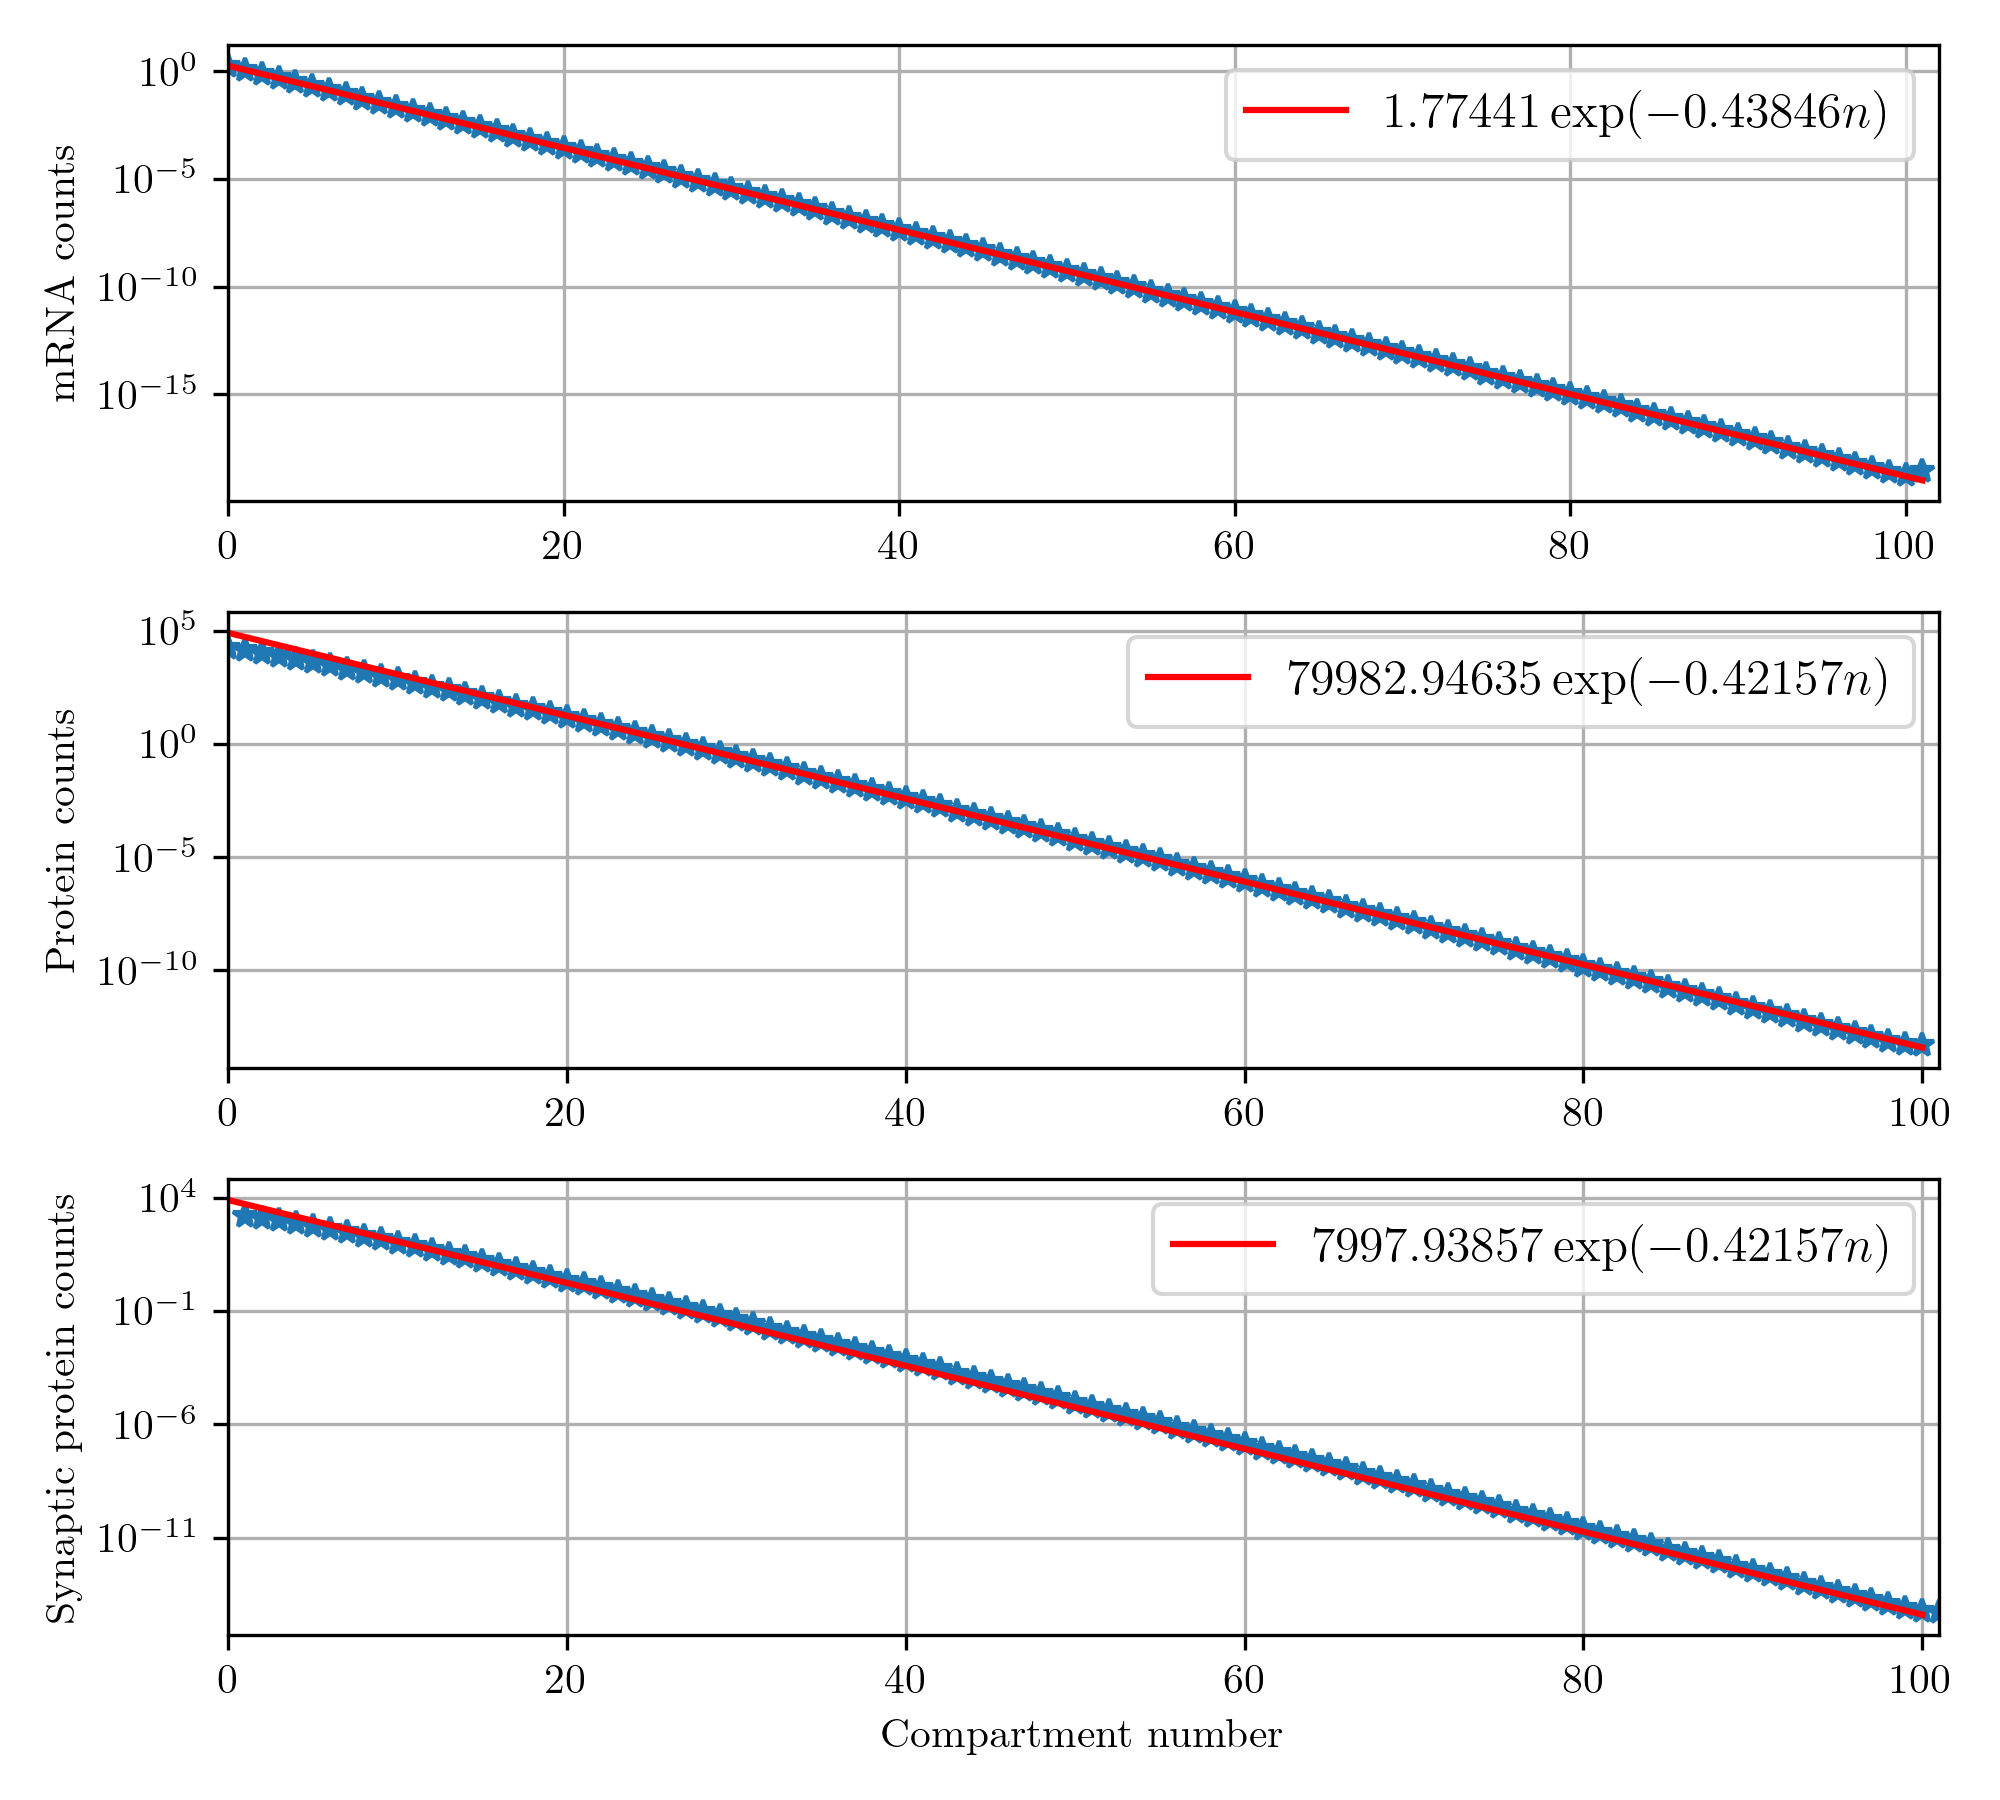
\includegraphics[width=12cm]{img/linear_model_decays.png}
  \end{center}  
  \caption{Stationary distributions of molecule numbers in linear (no forks) model with one synapse per dendritic segment. Note how the decay exponent for the synaptic protein counts matches that of the dendritic protein counts (the bottom and the middle panels respectively).}
  \label{fig:linear_model_decays}
\end{figure}

\begin{figure}
  \begin{center}
    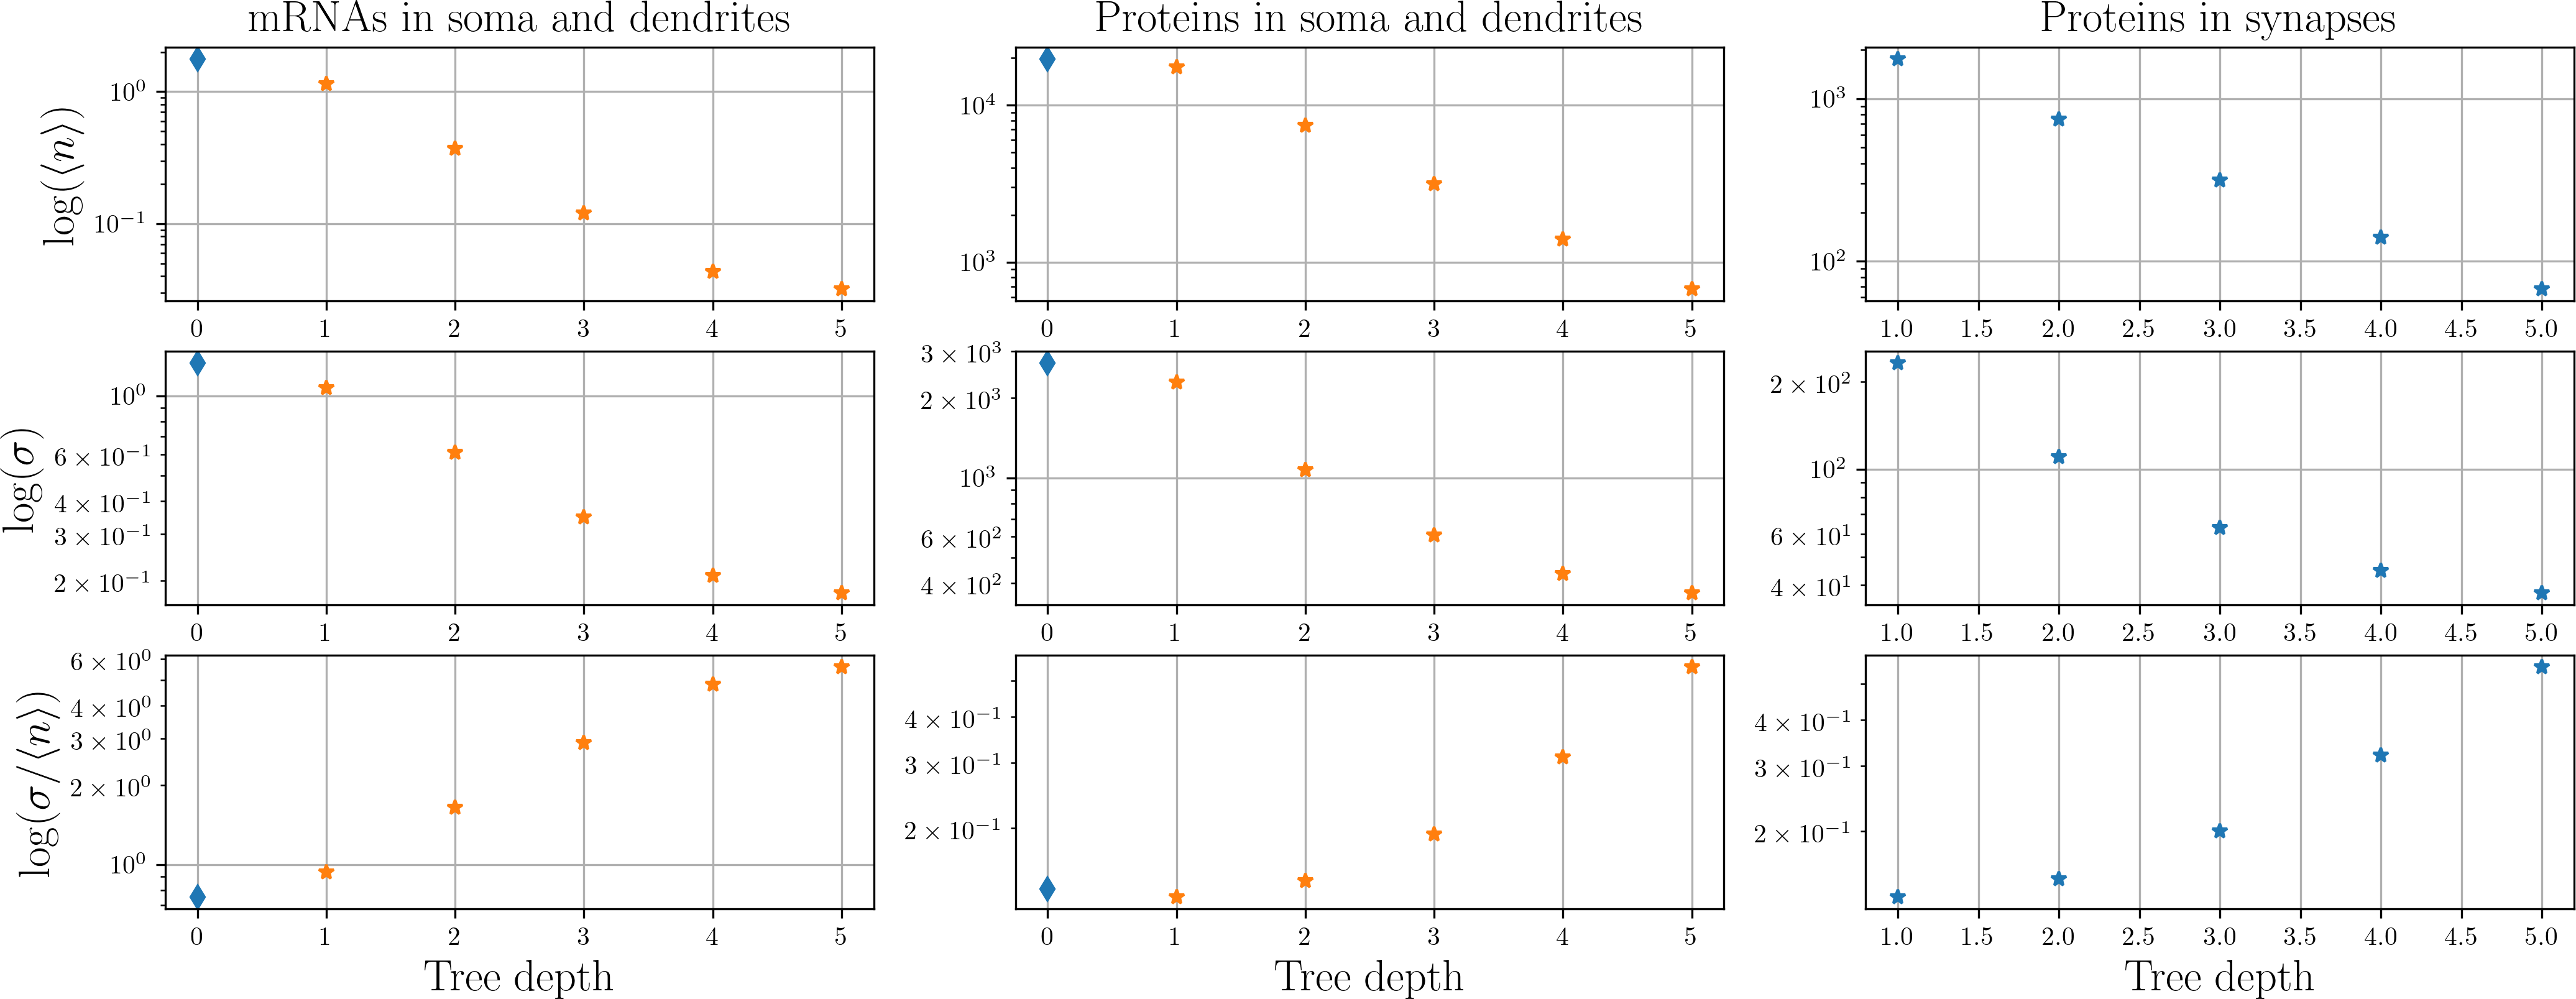
\includegraphics[width=15cm]{img/4_forks_plots_trimmed.png}
  \end{center}
    \caption{Protein and mRNA counts' stationary expectations and standard deviations in symmetric model similar to the simple model (same parameters and two synapses on every dendritic segment), but with {\bf four} branching points in each full path up the dendritic tree.}
  \label{fig:4_forks_noise}
\end{figure}

\begin{figure}
  \begin{center}
    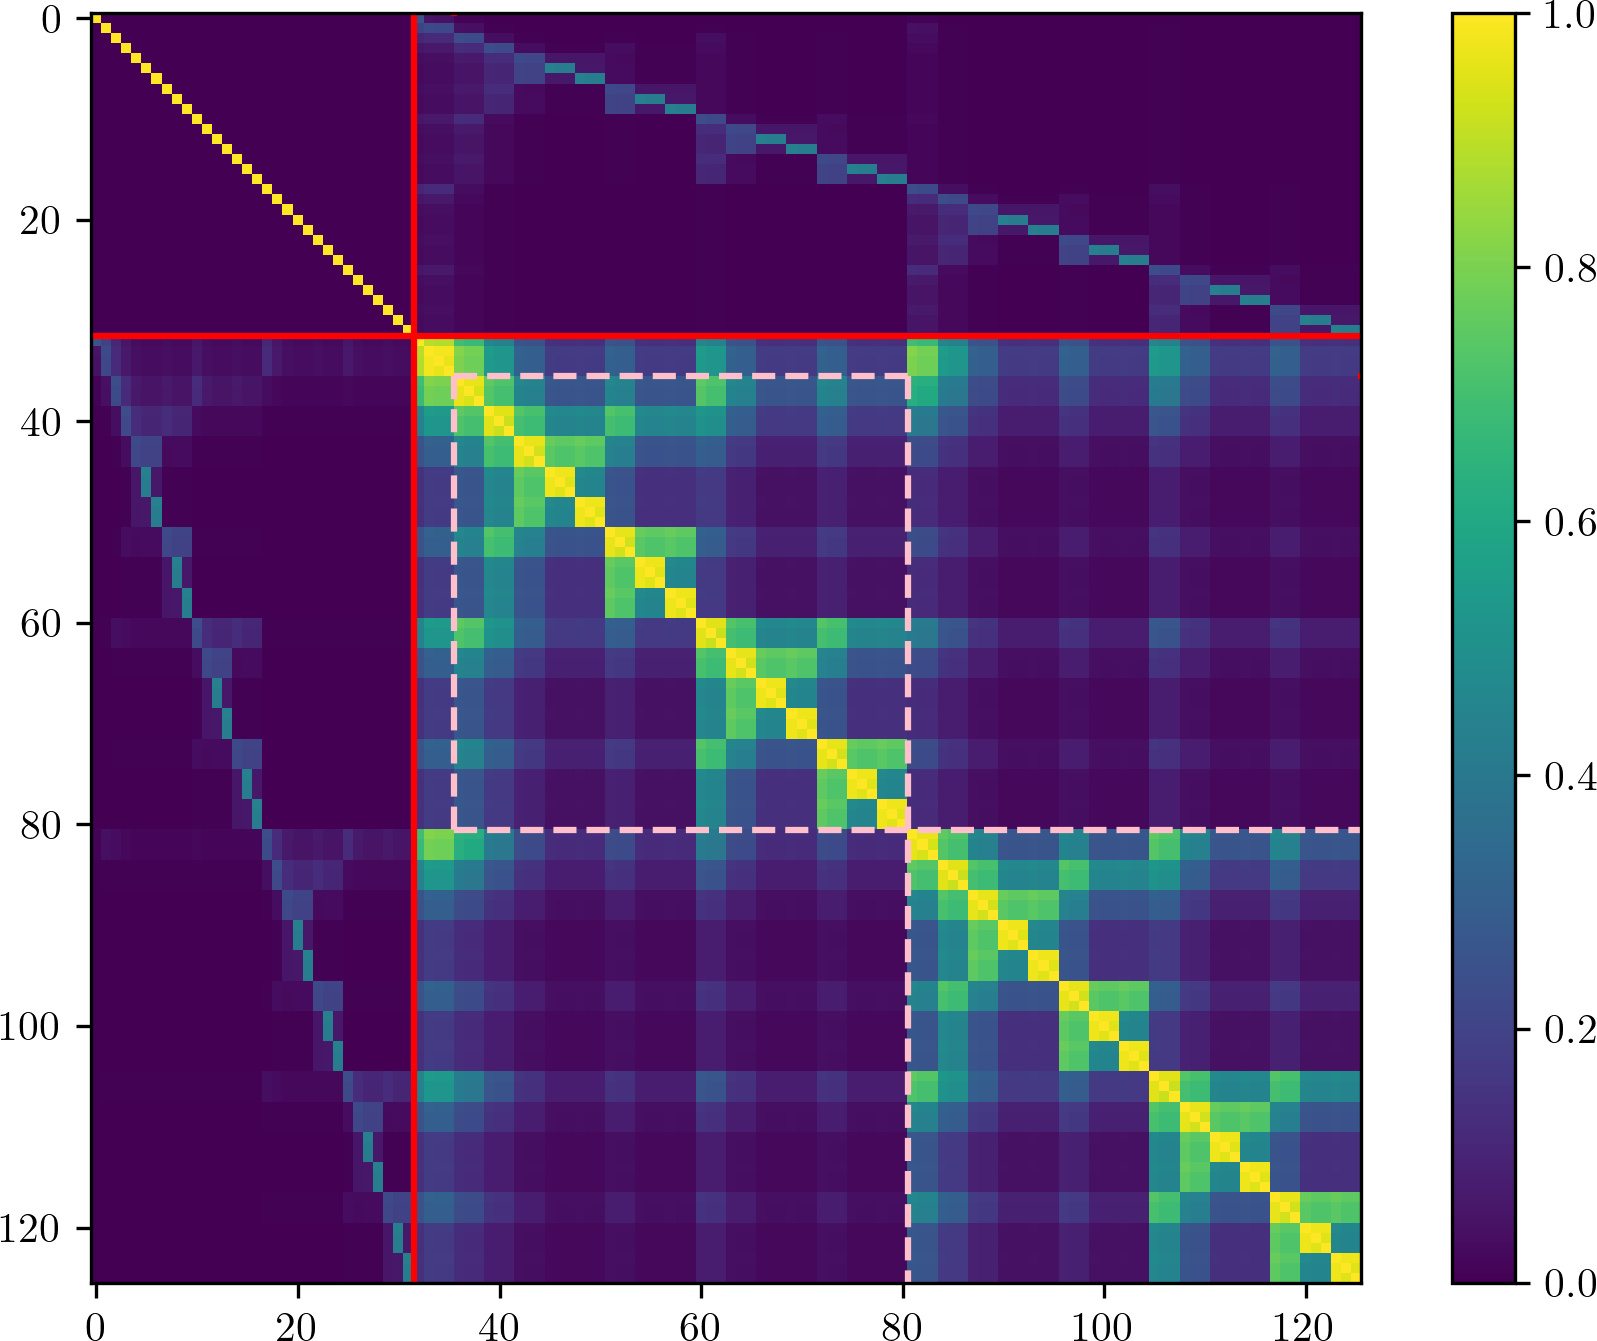
\includegraphics[width=15cm]{img/4_forks_pearson_correlations.png}
  \end{center}
    \caption{Pearson correlations in the model similar to the simple model (same parameters and two synapses on every dendritic segment), but with {\bf four} branching points in each full path up the dendritic tree. Vertical and horizontal red lines separate the plane in four regions. The square region that contains the origin (0,0) shows mRNA-mRNA Pearson correlations in all compartments; the upper right and the lower left rectangles are responsible for mRNA-protein correlations (note that the matrix is, of course, symmetric); and the lower right square corresponds to protein-protein correlations in all compartments. The dashed pink squares span the two parts of the tree that stem from the first branching point and, due to symmetry, are identical. The high-correlation $3\times3$ squares on the diagonal are produced by dendritic segments (at the top left corner of each square) and the two attached synapses.}
  \label{fig:4_forks_pearson_correlations}
\end{figure}


\section{Nonstationary problem}
\subsection{First order}\label{subsec:o1_nonstat_problem}
In this section we no longer assume stationarity and consider the dynamics of the expectations. When in the PDE for the generating function the coefficients corresponding to certain $x$ are collected and equated, in first order one gets the following inhomogeneous linear system of first-order ODEs
\begin{equation}
\frac{d\boldsymbol{\mathcal G}^{(1)}(t)}{dt} = -\mathbf A \boldsymbol{\mathcal G}^{(1)}(t) + \mathbf b,
\end{equation}
whose general solution is given by
\begin{equation}\label{general_solution}
\boldsymbol{\mathcal G}^{(1)}(t) = \mathbf A^{-1}\mathbf b + \mathrm e^{-\mathbf A t}\mathbf c,
\end{equation}
where the vector $\mathbf v$ is given by
\begin{equation}\label{rhs_vector}
  b_i=\lambda^+_1N\delta_{i1}
\end{equation}
and $\mathbf c$ is the vector determined by the initial conditions. The first term in the above expression determines the stationary expectations while the second term defines the relaxation dynamics from a given initial state.

To quantify the characteristic relaxation times we need to find the spectrum of $\mathbf A$, and it is convenient to use eigen decomposition as follows. Suppose $\mathbf S$ is the matrix consisting of the eigenvectors of $\mathbf A$, i.e. a transition matrix to a basis in which $\mathbf A$ is diagonal, i.e.
\begin{equation} \label{A_tilde_def}
  \tilde{\mathbf A} := \mathbf S^{-1}\mathbf A\mathbf S = \text{diag}(\lambda_1, \lambda_2, ..., \lambda_n).
\end{equation}
Multiplying both sides of the equation (\ref{general_solution}) by $\mathbf S^{-1}$ and inserting $\mathbf S\mathbf S^{-1}$ in the matrix-vector multiplication on the right-hand side gives
\begin{equation*}
  \mathbf S^{-1} \boldsymbol{\mathcal G}^{(1)}(t) = \mathbf S^{-1}\mathbf A^{-1}\mathbf S\mathbf S^{-1}\mathbf b + \mathbf S^{-1}\mathrm e^{-\mathbf A t}\mathbf S\mathbf S^{-1}\mathbf c,
\end{equation*}
from which using (\ref{A_tilde_def}) we obtain
\begin{equation}
  \boldsymbol{\mathcal G}^{(1)}(t) = \mathbf S\tilde{\mathbf A}^{-1}\mathbf S^{-1}\mathbf b + \mathbf S\mathrm e^{-\tilde{\mathbf A} t}\mathbf S^{-1}\mathbf c.
\end{equation}
Computing the right-hand side of the above equation can be done as follows. First we note that%$\mathbf S\tilde{\mathbf A}\mathbf S^{-1}\mathbf b$ is done as follows
\begin{equation}
  \mathbf S\tilde{\mathbf A}^{-1}\mathbf S^{-1} = \tilde{\mathbf A}^{-1} + [\mathbf S, \tilde{\mathbf A}^{-1}]\mathbf S^{-1},
\end{equation}
where the commutator $[\mathbf S, \tilde{\mathbf A}^{-1}]$ is given by
\begin{equation}
  [\mathbf S, \tilde{\mathbf A}^{-1}]_{ij} = [\mathbf S, \text{diag}(\lambda_1^{-1}, \lambda_2^{-1}, ... , \lambda_n^{-1})]_{ij} = (\lambda_k^{-1}-\lambda_i^{-1})S_{ij}
\end{equation}
where $\{\lambda_i\}$ are the eigenvales of $\mathbf A$. Similarly,
\begin{equation}
  \mathbf S\mathrm e^{-\tilde{\mathbf A} t}\mathbf S^{-1} = \text{diag}(\mathrm e^{-\lambda_1t}, \mathrm e^{-\lambda_2t},\dots,\mathrm e^{-\lambda_nt}) + [\mathbf S, \mathrm e^{-\tilde{\mathbf A} t}]\mathbf S^{-1},
\end{equation}
where
\begin{equation}
  [\mathbf S, \mathrm e^{-\tilde{\mathbf A} t}]_{ij} = (\mathrm e^{-\lambda_jt}-\mathrm e^{-\lambda_it})S_{ij}.
\end{equation}
Recalling the expression for $\mathbf b$ (\ref{rhs_vector}) we arrive to
\begin{multline}\label{nonstat_expectations_result}
  \mathcal G^{(1)}_i(t) = \lambda_1^+N\sum_{k=1}^{d_1}\lambda_k^{-1}S_{ik}\mathbf S^{-1}_{k1} + \mathrm e^{-\lambda_it}c_i + \sum_{k,l}(\mathrm e^{-\lambda_kt}-\mathrm e^{-\lambda_it})S_{ik}\mathbf S^{-1}_{kl}c_l \\
  = \lambda_1^+N\sum_{k=1}^{d_1}\lambda_k^{-1}S_{ik}\mathbf S^{-1}_{k1} + \sum_{k=1}^{d_1}\mathrm e^{-\lambda_kt}S_{ik}\sum_{l=1}^{d_1}\mathbf S^{-1}_{kl}c_l,
\end{multline}
from where
\begin{equation}
\mathcal G^{(1)}_i(\infty) = \mathbf A^{-1}\mathbf b = \lambda_1^+N\sum_{k=1}^{d_1}\lambda_k^{-1}S_{ik}\mathbf S^{-1}_{k1},
\end{equation}
which expresses the stationary expectations through the eigen decomposition of $\mathbf A$.
The constant vector $\mathbf c$ can be found from (\ref{nonstat_expectations_result}) at $t=0$ as
\begin{equation}\label{o1_constants_definition}
  \mathbf c = \boldsymbol{\mathcal G}^{(1)}(0) - \boldsymbol{\mathcal G}^{(1)}(\infty).
\end{equation}

Finally, combining the expressions (\ref{nonstat_expectations_result}) and (\ref{o1_constants_definition}) we arrive to the following expression for the first-order expectations\footnote{Note that to compute the expectations numerically we use (\ref{nonstat_expectations_result}) and (\ref{o1_constants_definition}) instead of (\ref{nonstat_expectations_final_result}), as it is usually more optimal to separate time-dependent and time-independent terms.}
\begin{equation}\label{nonstat_expectations_final_result}
  \mathcal G^{(1)}_i(t) = \lambda_1^+N\sum_{k=1}^{d_1}\frac{1-\mathrm e^{-\lambda_kt}}{\lambda_k}S_{ik}\mathbf S^{-1}_{k1} + \sum_{k=1}^{d_1}\mathrm e^{-\lambda_kt}S_{ik}\sum_{l=1}^{d_1}\mathbf S^{-1}_{kl}\mathcal G^{(1)}_l(t=0).
\end{equation}

The comparison of the above predictions with the results of the corresponding Gillespie simulation is shown in Fig.\ref{fig:Gillespie_simulation}.

\begin{figure}
  \begin{center}
    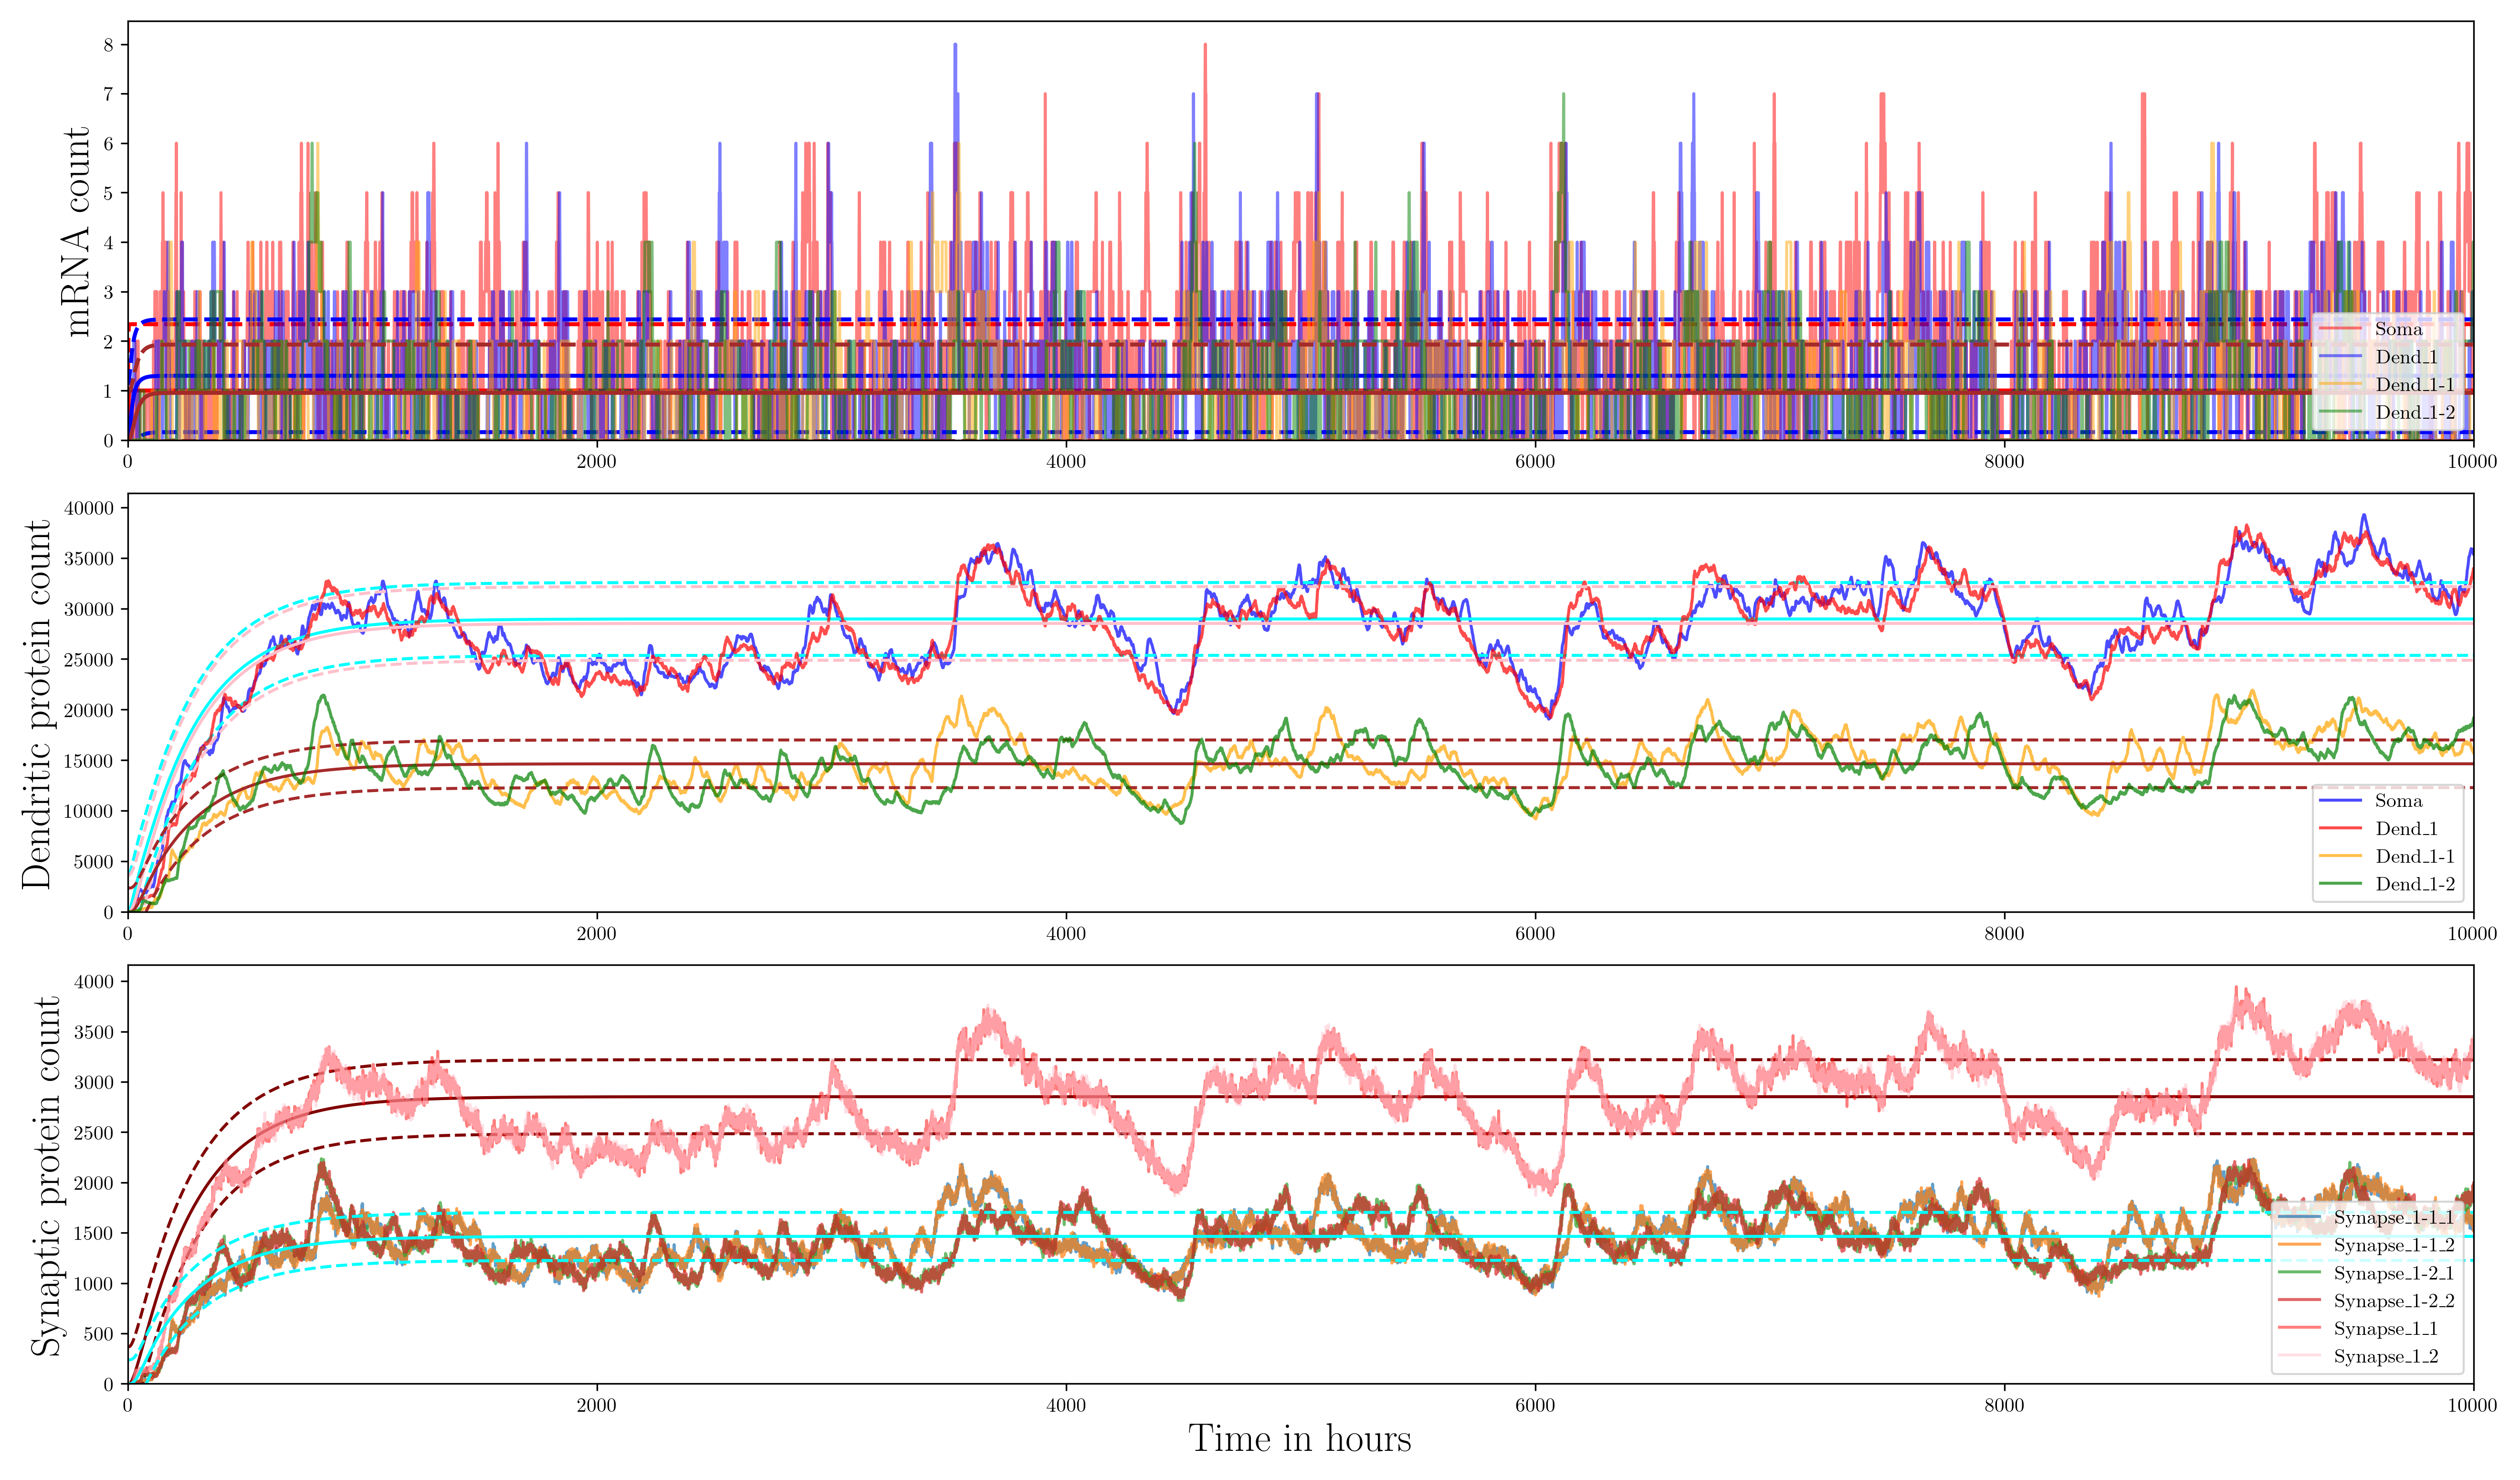
\includegraphics[width=15cm]{img/protein_numbers.png}
  \end{center}  
  \caption{Comparison of theoretical predictions with Gillespie simulation starting from zero active genes, zero mRNAs and zero proteins. \textcolor{red}{Note that standard deviations are shown at their stationary values.}}
  \label{fig:Gillespie_simulation}
\end{figure}

\subsection{Second order}
When in the PDE for the generating function the coefficients corresponding to certain pairs $x_ix_j$ are collected and equated, one gets an inhomogeneous linear system of first-order ODEs for $\boldsymbol{\mathcal G^{(2)}}$ of the form
\begin{equation}\label{o2_nonstat_ODE}
  \frac{d\boldsymbol{\mathcal G}^{(2)}(t)}{dt} = \mathbf D\boldsymbol{\mathcal G}^{(1)}(t) - \mathbf C\boldsymbol{\mathcal G}^{(2)}(t),
\end{equation}
where $\boldsymbol{\mathcal G}^{(2)}(t)$ should now be understood as a vector consisting of all independent\footnote{$\boldsymbol{\mathcal G}^{(2)}(t)$ was defined above as a symmetric matrix.} entries of the $\boldsymbol{\mathcal G}^{(2)}$ matrix discussed above ordered in a certain way\footnote{As discussed in Appendix \ref{app:Computational_optimisations}, it makes sense to group the entries of the $\boldsymbol{\mathcal G}^{(2)}$ matrix as gene-gene, gene-mRNA, gene-protein, mRNA-mRNA, mRNA-protein, protein-protein. This grouping simplifies the matrix $\mathbf C$, but, in principle, the 1-d arrangement of $\boldsymbol{\mathcal G}^{(2)}$ elements is arbitrary.}.

The general solution to the system of ODEs (\ref{o2_nonstat_ODE}) is given by
\begin{equation} \label{o2_nonstat_general_solution}
  \boldsymbol{\mathcal G}^{(2)}(t) = \mathrm e^{-\mathbf C t}\left(\boldsymbol{\mathcal G}^{(2)}(t=0) + \int_0^t\mathrm e^{\mathbf C\tau}\mathbf D\boldsymbol{\mathcal G}^{(1)}(\tau)d\tau\right),
\end{equation}
and, as in Section \ref{subsec:o1_nonstat_problem}, to make its computation tractable, we use eigen decomposition, denoting a matrix consisting of the $\mathbf C$'s eigenvectors as $\mathbf T$, which implies that
\begin{equation} \label{diagonalisation}
  \mathbf C = \mathbf T \tilde{\mathbf C} \mathbf T^{-1},
\end{equation}
where $\tilde{\mathbf C} = \text{diag}(\{\lambda^{(2)}_i|i=1,\dots,d_2\})$, with $d_2$ being the number of unordered pairs of variables (number of all second moments) and $\{\lambda^{(2)}_i|i=1,\dots,d_2\}$ being an ordered set of all eigenvalues of the matrix $\mathbf C$. Substituting (\ref{diagonalisation}) to (\ref{o2_nonstat_general_solution}) gives
\begin{multline} \label{nonstationary_o2_solution}
  \boldsymbol{\mathcal G}^{(2)}(t) = \mathbf T\mathrm e^{-\tilde{\mathbf C}t}\mathbf T^{-1}\left(\boldsymbol{\mathcal G}^{(2)}(t=0) + \int_0^t\mathbf T\mathrm e^{\tilde{\mathbf C}\tau}\mathbf T^{-1}\mathbf D\boldsymbol{\mathcal G}^{(1)}(\tau)d\tau\right)\\
  = \mathbf T\mathrm e^{-\tilde{\mathbf C}t}\left(\mathbf T^{-1}\boldsymbol{\mathcal G}^{(2)}(t=0) + \int_0^t\mathrm e^{\tilde{\mathbf C}\tau}\mathbf T^{-1}\mathbf D\boldsymbol{\mathcal G}^{(1)}(\tau)d\tau\right),
\end{multline}
from which\footnote{The integral
\begin{equation}
  I_{j\eta}(t) = \int_0^t\mathrm e^{-\lambda^{(2)}_j(t-\tau)}\mathcal G^{(1)}_\eta(\tau)d\tau
\end{equation}
from the expression (\ref{nonstationary_o2_solution}) can be numerically computed using the fact that it satisfies the following ODE
\begin{equation*}
  \frac{dI_{j\eta}}{dt} = \mathcal G^{(1)}_\eta(t) - \lambda_j^{(2)}I_{j\eta}(t),
\end{equation*}
which relates the values of the integral at the adjacent time steps as
\begin{equation*}
  I_{j\eta}(t+\Delta t) = I_{j\eta}(t) + \left(\mathcal G^{(1)}_\eta(t) - \lambda^{(2)}_jI_{j\eta}(t)\right)\Delta t,
\end{equation*}
which can be computed without additional loops in the main loop over time (no need to recompute the integral on every time step, just add the above correction to the previous integral value).
}
\begin{multline} \label{nonstationary_o2_solution}
  G^{(2)}_i(t) = \sum_{j=1}^{d_2}\mathrm e^{-\lambda^{(2)}_jt}T_{ij}\left\{\sum_{s=1}^{d_2}\mathbf T^{-1}_{js}\mathcal G^{(2)}_s(t=0) + \int_0^t\mathrm e^{\lambda^{(2)}_j\tau}\sum_{k=1}^{d_2}\mathbf T^{-1}_{jk}\sum_{\eta=1}^{d_1}D_{k\eta}\mathcal G^{(1)}_\eta(\tau)d\tau\right\}\\
  = \sum_{j=1}^{d_2}T_{ij}\left\{\mathrm e^{-\lambda^{(2)}_jt}\sum_{s=1}^{d_2}\mathbf T^{-1}_{js}\mathcal G^{(2)}_s(t=0) + \sum_{\eta=1}^{d_1}\sum_{k=1}^{d_2}\mathbf T^{-1}_{jk}D_{k\eta}\int_0^t\mathrm e^{-\lambda^{(2)}_j(t-\tau)}\mathcal G^{(1)}_\eta(\tau)d\tau\right\}.
\end{multline}
Using the expression (\ref{nonstat_expectations_result}), the integral above is evaluated as
\begin{equation}
  \int_0^t\mathrm e^{\lambda_j^{(2)}\tau}\mathcal G^{(1)}_\eta(\tau)d\tau = \frac{\mathrm e^{\lambda_j^{(2)}t} - 1}{\lambda^{(2)}_j}\mathcal G_\eta^{(1)}(t=\infty) + \sum_{\mu=1}^{d_1}\frac{\mathrm e^{(\lambda^{(2)}_j-\lambda_\mu)t}-1}{\lambda^{(2)}_j-\lambda_\mu}S_{\eta\mu}\sum_{\nu=1}^{d_1}\mathbf S^{-1}_{\mu\nu}c_\nu,
\end{equation}
and finally
\begin{multline}
  \mathcal G^{(2)}_i(t) =  \sum_{j=1}^{d_2}\mathrm e^{-\lambda^{(2)}_jt}T_{ij}\Bigg\{\sum_{s=1}^{d_2}\mathbf T^{-1}_{js}\mathcal G^{(2)}_s(t=0) + \sum_{k=1}^{d_2}\mathbf T^{-1}_{jk}\sum_{\eta=1}^{d_1}D_{k\eta}\Bigg(\frac{\mathrm e^{\lambda_j^{(2)}t} - 1}{\lambda^{(2)}_j}\mathcal G_\eta^{(1)}(t=\infty)\\
  + \sum_{\mu=1}^{d_1}\frac{\mathrm e^{(\lambda^{(2)}_j-\lambda_\mu)t}-1}{\lambda^{(2)}_j-\lambda_\mu}S_{\eta\mu}\sum_{\nu=1}^{d_1}(\mathbf S^{-1})_{\mu\nu}c_\nu\Bigg)\Bigg\},
\end{multline}
or
\begin{multline} \label{nonstat_covar}
  \mathcal G^{(2)}_i(t) =  \sum_{j=1}^{d_2}T_{ij}\Bigg\{\mathrm e^{-\lambda^{(2)}_jt}\sum_{s=1}^{d_2}\mathbf T^{-1}_{js}\mathcal G^{(2)}_s(t=0) + \frac{1 - \mathrm e^{-\lambda^{(2)}_jt}}{\lambda^{(2)}_j}\sum_{\eta=1}^{d_1}\left(\sum_{k=1}^{d_2}\mathbf T^{-1}_{jk}D_{k\eta}\right)\mathcal G_\eta^{(1)}(t=\infty)\\
  + \sum_{\mu=1}^{d_1}\frac{\mathrm e^{-\lambda_\mu t}-\mathrm e^{-\lambda^{(2)}_jt}}{\lambda^{(2)}_j-\lambda_\mu}\left(\sum_{\zeta=1}^{d_1}\left(\sum_{k=1}^{d_2}\mathbf T^{-1}_{jk}D_{k\zeta}\right)S_{\zeta\mu}\right)\sum_{\nu=1}^{d_1}(\mathbf S^{-1})_{\mu\nu}c_\nu\Bigg\},
\end{multline}
or, substituting $c_\nu$ from (\ref{o1_constants_definition})
\begin{multline}
  \mathcal G^{(2)}_i(t) = \sum_{\eta=1}^{d_1}\sum_{k=1}^{d_2}\sum_{j=1}^{d_2}\frac{T_{ij}\mathbf T^{-1}_{jk}}{\lambda^{(2)}_j}D_{k\eta}\mathcal G_\eta^{(1)}(t=\infty) +\\
  \sum_{j=1}^{d_2}\mathrm e^{-\lambda^{(2)}_jt}\left(\sum_{s=1}^{d_2}T_{ij}\mathbf T^{-1}_{js}\mathcal G^{(2)}_s(t=0) - \sum_{\eta=1}^{d_1}\sum_{k=1}^{d_2}\frac{T_{ij}\mathbf T^{-1}_{jk}}{\lambda^{(2)}_j}D_{k\eta}\mathcal G_\eta^{(1)}(t=\infty)\right) +\\
  \sum_{j=1}^{d_2}\mathrm e^{-\lambda^{(2)}_jt}T_{ij}\sum_{\mu=1}^{d_1}\frac{\mathrm e^{(\lambda^{(2)}_j-\lambda_\mu)t}-1}{\lambda^{(2)}_j-\lambda_\mu}\sum_{k=1}^{d_2}\mathbf T^{-1}_{jk}\sum_{\zeta=1}^{d_1}D_{k\zeta}S_{\zeta\mu}\sum_{\nu=1}^{d_1}(\mathbf S^{-1})_{\mu\nu}\left(\mathcal G_\nu^{(1)}(t=0) - \mathcal G_\nu^{(1)}(t=\infty)\right).
\end{multline}

The last expression is written in the form that clarifies the meanings of different terms. Indeed, the first term in the above expression gives stationary values of $\boldsymbol{\mathcal G}^{(2)}$, the second terms gives the decay dynamics of $\boldsymbol{\mathcal G}^{(2)}$ if $\boldsymbol{\mathcal G}^{(1)}$ are set at their stationary values, finally the last term is important if the first-order moments are themselves away from stationarity.

For numerical evaluation of $\boldsymbol{\mathcal G}^{(2)}(t)$ we use the expression (\ref{nonstat_covar}) in which, if $\lambda^{(2)}_j-\lambda_\mu=0$ we evaluate the fraction as a limit
\begin{equation}
  \lim_{\lambda^{(2)}_j-\lambda_\mu\to 0}\frac{\mathrm e^{-\lambda_\mu t}-\mathrm e^{-\lambda^{(2)}_jt}}{\lambda^{(2)}_j-\lambda_\mu} = t\mathrm e^{-\lambda^{(2)}_jt},
\end{equation}
which corresponds to a situation where some dynamical modes of $\boldsymbol{\mathcal G}^{(1)}$ and $\boldsymbol{\mathcal G}^{(2)}$ decay together with identical rates.

\subsubsection{Note on initial conditions}
\textcolor{red}{It is important to understand that the initial conditions $\boldsymbol{\mathcal G}^{(1)}(t=0)$ and $\boldsymbol{\mathcal G}^{(2)}(t=0)$ should be consistent with their physical meanings and with each other.} Indeed, if this is not the case, the expectation of the number of active genes may be set higher than the total number of gene copies, or, say, a negative value for the expected mRNA number may be set. Moreover, low $\mathcal G_{ii}^{(2)}(t=0)$ at high $\mathcal G_i^{(1)}(t=0)$ results in negative variances.

The initial conditions $\boldsymbol{\mathcal G}^{(1)}(t=0)$ and $\boldsymbol{\mathcal G}^{(2)}(t=0)$ should be set in a way consistent with some underlying probability distribution from which these quantities can arise. It is necessary (and, possibly, sufficient) to check that the covariance matrix is positive semi-definite. 

\appendix \label{app:Computational_optimisations}
\section{Computational optimisations}
It is important to note that gene activation/deactivation is completely independent from mRNA/protein dynamics, mRNA dynamics solely depends on gene dynamics, and protein dynamics only depends on mRNA dynamics. This allows separating the whole first-order system of linear equations to one equation corresponding to gene dynamics, 1+(number of dendritic segments) equations for mRNA dynamics and 1+(number of dendritic segments) + (number of synapses) equations for protein dynamics. In this setting, protein dynamics can be found by solving equation for gene dynamics and substituting the result to the r.h.s. of the mRNA equations, whose results should then be substituted to the r.h.s. of protein equations.

Similar idea holds for the second-order equations (for covariances), which can be separated as \{(gene-gene), (gene-mRNA), (gene-protein), (mRNA-mRNA), (mRNA-protein), (protein-protein)\}. The computational cost is then defined mainly by the (protein-protein) part, which requires the largest matrix inversion, but, if protein-protein correlations are unfeasible to compute, one can still obtain something that is feasible (e.g. mRNA-mRNA correlations), which would not be possible if the system of equations was inseparable in the above sense.

Of course, these optimisations do not change the exponent of the problems' computational complexity, but they significantly decrease the constant in computational time and memory consumption.

\bibliographystyle{unsrt}
\bibliography{bibliography.bib}

\end{document}
